\documentclass{beamer}
%[aspectratio=169]   \usepackage[czech]{babel}
\usepackage{apo-lecture-en}
\usepackage{pdfpages}
\usepackage{pdfcomment}
\usepackage{listings}
\usepackage{array,multirow}

\subtitle{Lecture 05. Pipelined Instruction Execution}
\author{Pavel Píša \phantom{xxxxxxx} Petr Štěpán \\ \small\texttt{pisa@fel.cvut.cz} \phantom{x} \small\texttt{stepan@fel.cvut.cz} \\
\phantom{xxxxxxxxx} \\
License: CC-BY-SA}
\begin{document}

\maketitle

\section{Pipelined Execution}

\begin{frame}
\frametitle{The Goal of Today's Lecture}

\begin{itemize}
 \item Convert/extend CPU presented in the lecture 3 to the pipelined CPU design to make it faster
 \item The following instructions are considered for our CPU design: \texttt{add}, \texttt{sub}, \texttt{and}, \texttt{or}, \texttt{slt}, \texttt{addi}, \texttt{lw}, \texttt{sw}, and \texttt{beq}
 \item Instruction coding stays the same as well
\end{itemize}

\begin{table}
\footnotesize
\begin{tabular}{|m{0.4cm}|m{0.4cm}|m{1.0cm}|m{1.0cm}|m{0.4cm}|m{1.0cm}|m{1.0cm}|m{1.0cm}|m{0.4cm}|m{1.0cm}|}\hline
Typ & 31 & 30...25 & 24...21 & 20 & 19...15 & 14...12 & 11...8 & 7 & 6...0 \\ \hline
R & \multicolumn{2}{c|}{ fnct7 } & \multicolumn{2}{c|}{ rs2 } & rs1 & fnct3 &\multicolumn{2}{c|}{ rd } & opcode\\ \hline
I & \multicolumn{4}{c|}{ imm[11:0] } & rs1 & fnct3 &\multicolumn{2}{c|}{ rd } & opcode\\ \hline
S & \multicolumn{2}{c|}{ imm[11:5] } & \multicolumn{2}{c|}{ rs2 } & rs1 & fnct3 &\multicolumn{2}{c|}{ imm[4:0] } & opcode\\ \hline
B & imm [12] & imm [10:5]  & \multicolumn{2}{c|}{ rs2 } & rs1 & fnct3 & imm[4:1]& imm [11] & opcode\\ \hline
U & \multicolumn{6}{c|}{ imm[31:12] }  & \multicolumn{2}{c|}{ rd } & opcode\\ \hline
J & imm [20] & \multicolumn{2}{c|}{ imm[10:1] } & imm [11] & \multicolumn{2}{c|}{ imm[19:12] } & \multicolumn{2}{c|}{ rd } & opcode\\ \hline
\end{tabular}
\end{table}

\end{frame}

\begin{frame}
\frametitle{Single Cycle CPU with Memories (from Lecture 3)}
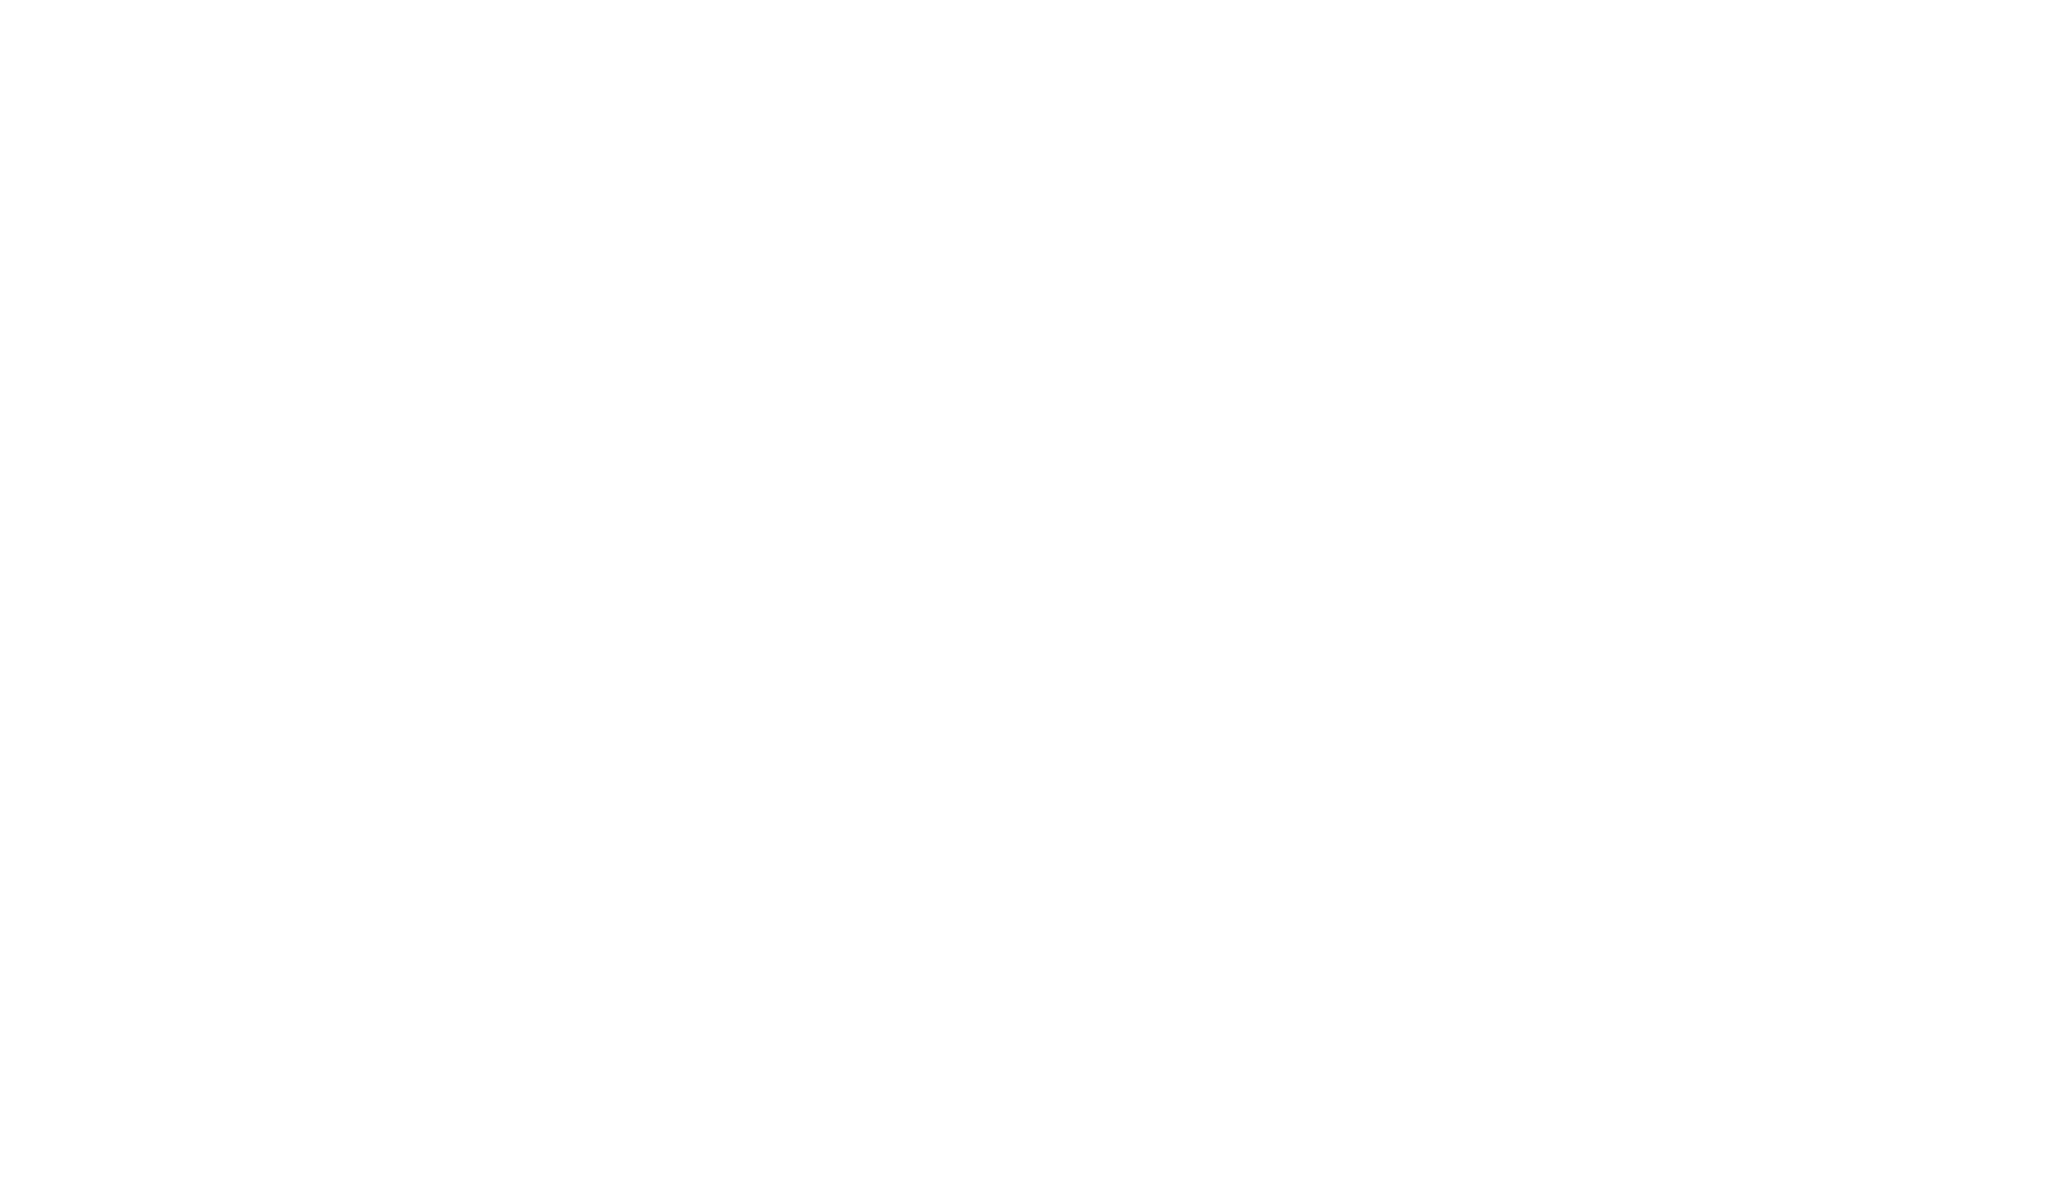
\includegraphics[width=0.95\textwidth]{single_cpu.pdf}
\end{frame}

\begin{frame}
\frametitle{The Throughput of a Single-cycle Processor Is Limited}

\begin{itemize}
 \item Maximum instructions per second $IPS = IC / T = IPC_{avk} \cdot f_{clk}$
 \item Limited by the longest signal path time from the previous registered value to the input of the register (critical path)
 \item In our design, the limitation is \texttt{lw} instruction execution
\end{itemize}

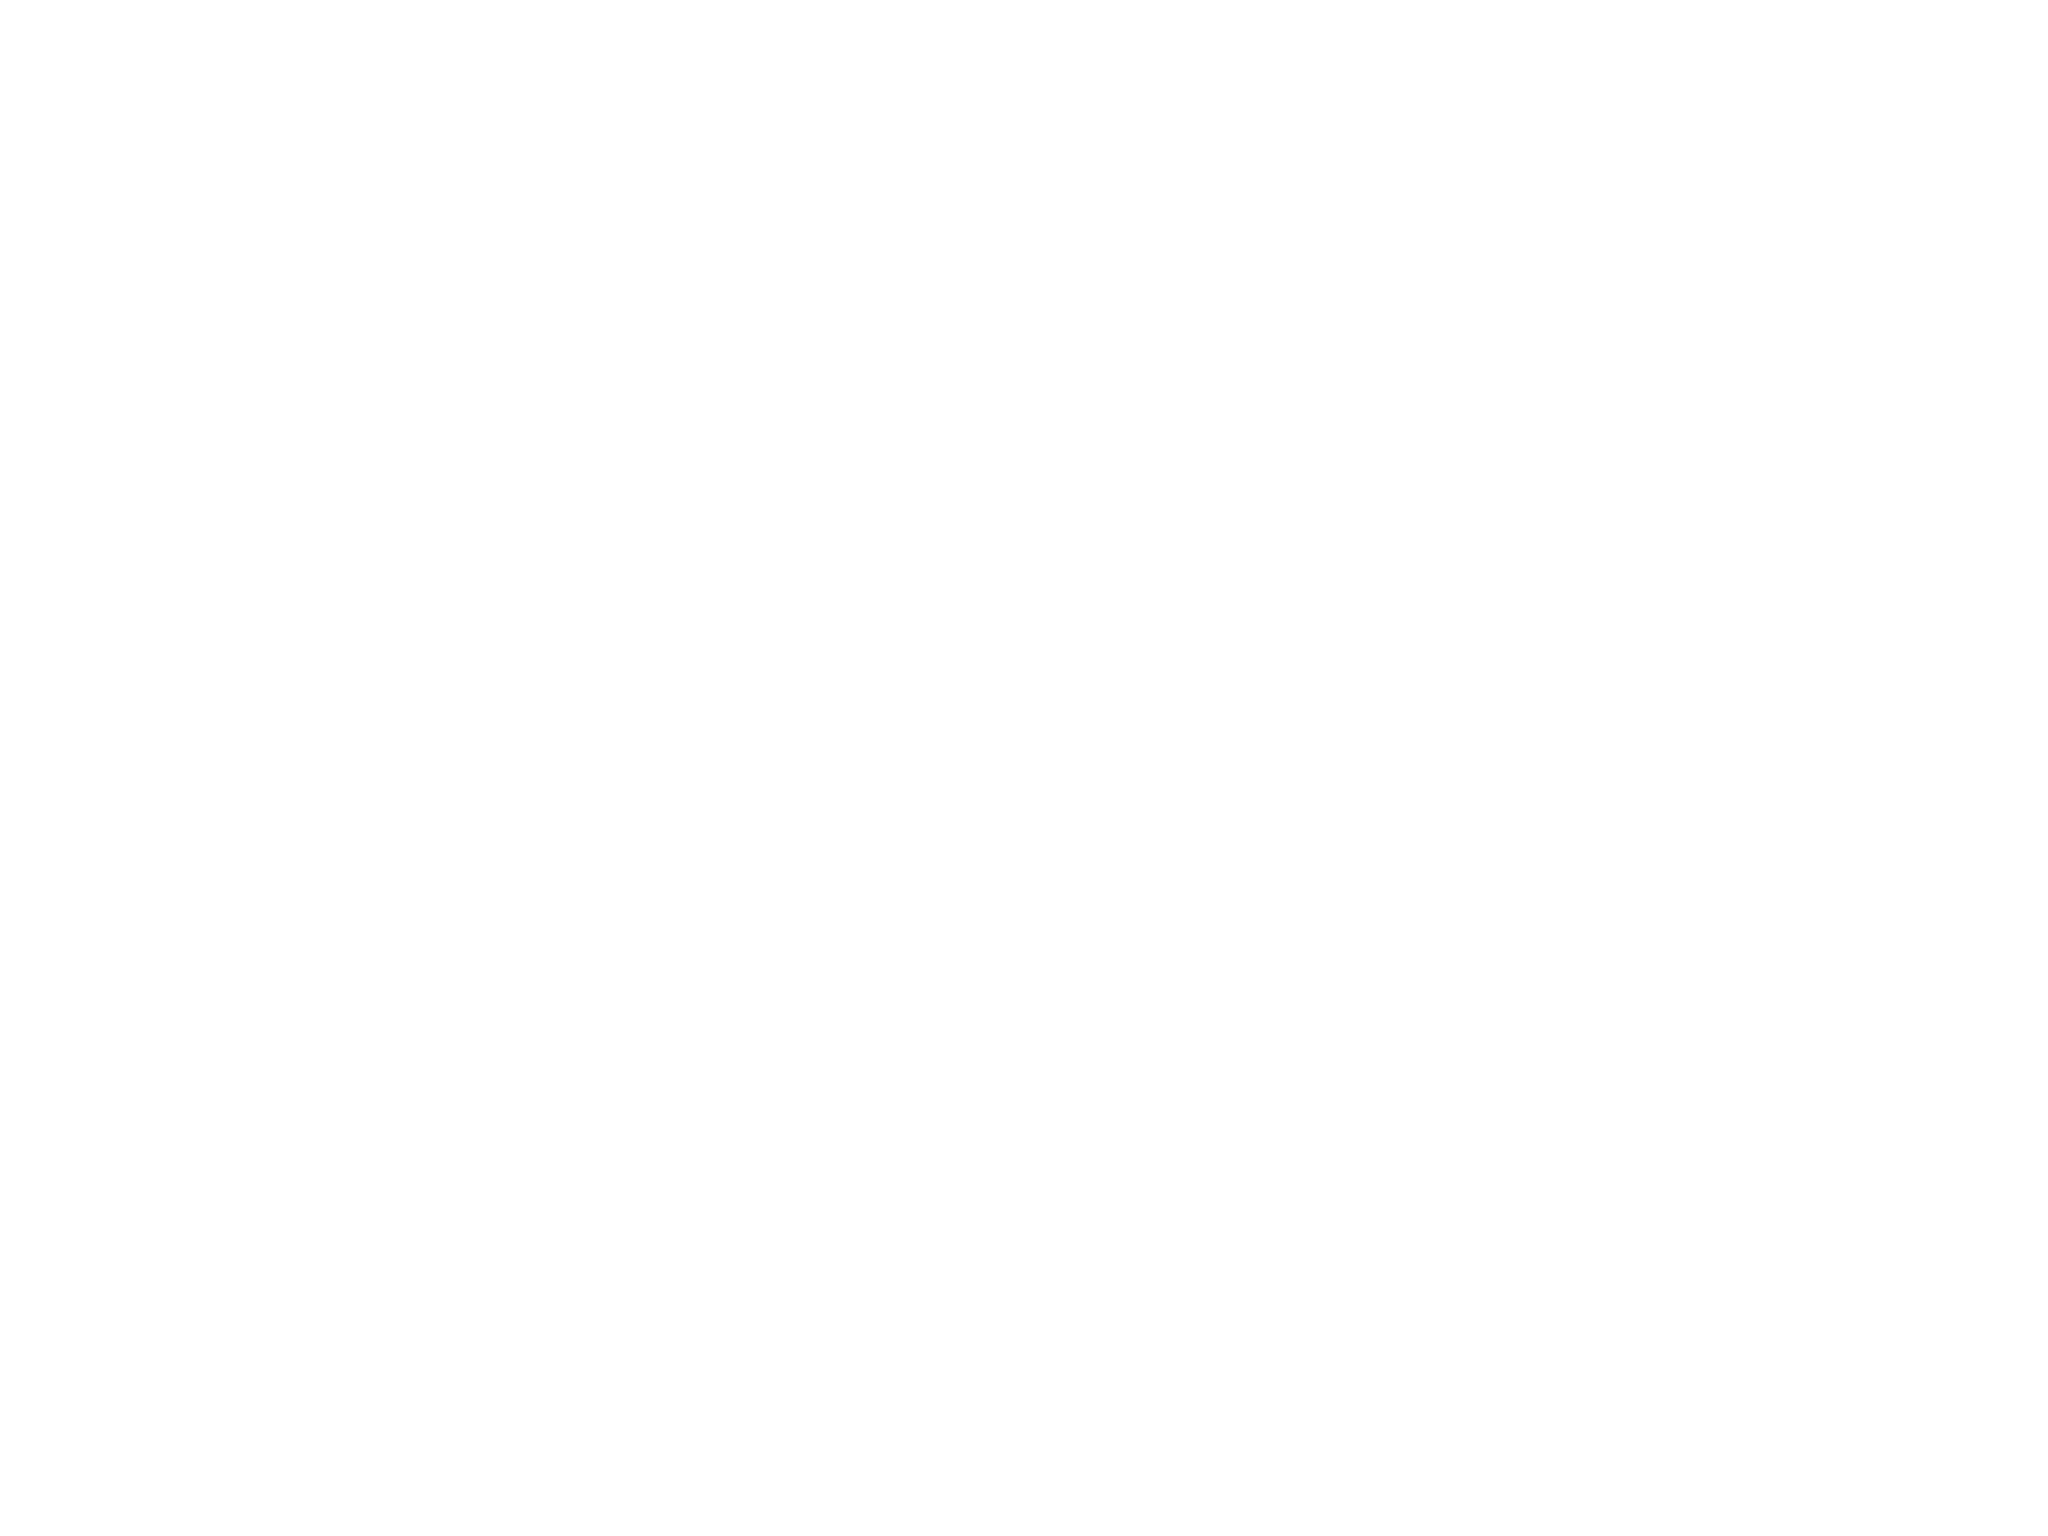
\includegraphics[width=0.92\textwidth]{cpu-time.pdf}
\end{frame}

\begin{frame}
\frametitle{Critical Path Limiting Throughput}

$f_{clk} = 1 / T_{C}$ where $T_{C}$ is the period of clock to process one cycle

\vskip 2 mm

$T_{C} = t_{PC} + t_{Mem} + t_{RFread} + t_{ALU} + t_{Mem} + t_{Mux} + t_{RFsetup}$

\vskip 2 mm

We consider the following times required for signal propagation

\vskip 2 mm

\begin{tabular}{l c r}
$t_{PC}$ & = & $30$ ns \\
$t_{Mem}$ & = & $300$ ns \\
$t_{RFread}$ & = & $150$ ns \\
$t_{ALU}$ & = & $200$ ns \\
$t_{Mux}$ & = & $20$ ns \\
$t_{RFsetup}$ & = & $20$ ns \\
\end{tabular}

\vskip 2 mm

$T_{C} = 1020$\,ns $\rightarrow$ $f_{clk max} = 980$\,kHz

\vskip 2 mm

$IPS = IC / T = IPC_{avg} \cdot f_{clk}$

\vskip 2 mm

$IPS = 1 \cdots 980e3 = 980\,000$ instructions per second

\end{frame}

\begin{frame}
\frametitle{Separate Instruction Fetch and Execution}

\begin{itemize}
 \item Fetching an instruction and execution of data load from memory ($2 \times t_{Mem}$) usually accounts for a significant part of the total cycle time
 \item It helps to reduce the cycle time if an instruction is already loaded in a previous cycle
\end{itemize}

\vskip 2 mm

{
\centering

\includegraphics[width=0.8\textwidth]{cpu_ifetch_exe.pdf}
}

\vskip 2 mm

\begin{enumerate}
 \item Instruction fetch and instruction counter increment $PC = PC + 4$
 \item The actual execution of the instruction in the following cycle
\end{enumerate}

\end{frame}

\begin{frame}
\frametitle{Non-Pielined Execution with Instructions Prefetching}
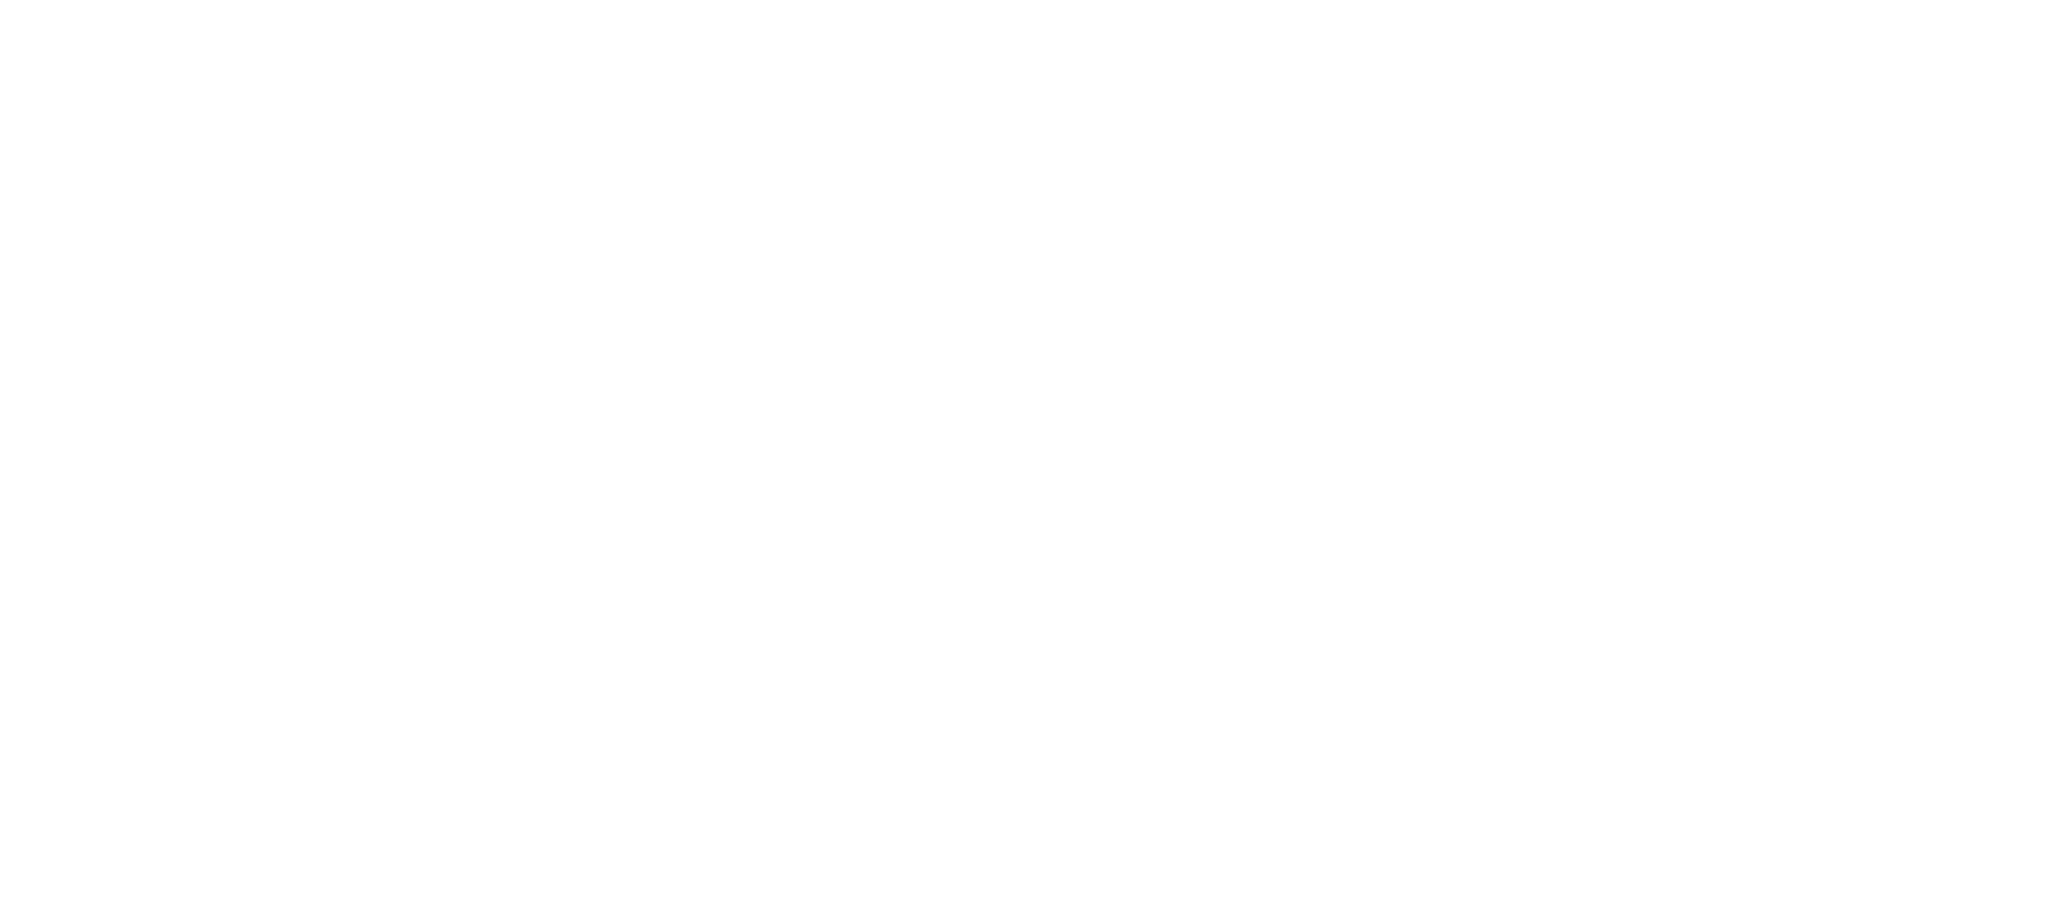
\includegraphics[width=0.95\textwidth]{cpu_clock.pdf}
\begin{itemize}
 \item $\downarrow$ in the figure represents the clock input active on the rising edge of the clock signal
\end{itemize}

\end{frame}

\begin{frame}
\frametitle{Critical Path in Case of Prefetching}

For the previously considered parameters

\vskip 2 mm

\begin{tabular}{l c r m{1 cm} l c r}
$t_{PC}$ & = & $30$ ns & & $t_{Mem}$ & = & $300$ ns \\
$t_{RFread}$ & = & $150$ ns  & & $t_{ALU}$ & = & $200$ ns \\
$t_{Mux}$ & = & $20$ ns  & & $t_{RFsetup}$ & = & $20$ ns \\
\end{tabular}

\vskip 2 mm

\begin{itemize}
 \item We consider $T_{C_{fetch}} = t_{PC} + t_{Mem}$ running in parallel with the execution of the preceding instruction
 \item $T_{C_{exec}} = t_{RFread} + t_{ALU} + t_{Mem} + t_{Mux} + t_{RFsetup}$
\end{itemize}

after substituting the values into the expressions

\begin{itemize}
 \item Consider $T_{C_{fetch}} = 30 + 300 = 330$\,ns
 \item $T_{C_{exec}} = 150 + 200 + 300 + 20 + 20 = 690$\,ns
 \item $T_{C_{fetch}} < T_{C_{exec}}$ so $T_{C} = T_{C_{exec}} = 690$\,ns
 \item $\rightarrow f_{C} = 1.45$\,MHz $\rightarrow IPS = 1\,450\,000$
\end{itemize}

Without modifications, the delay of the jump instructions (\texttt{beq}) will occur, see later in the lecture

\end{frame}

\section{Five-Stage Pipeline}

\begin{frame}
\frametitle{Pipelined Instruction Execution}

We will consider splitting instruction execution into five stages.

\vskip 2 mm

{
\centering
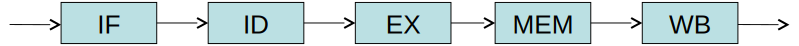
\includegraphics[width=0.9\textwidth]{cpu_pipe_stages.pdf}
}

\begin{enumerate}
 \item \textbf{IF} -- \textbf{Instruction Fetch} -- setup \textbf{PC} value to the memory address input, fetch the instruction and prepare $PC = PC + 4$ in parallel
 \item \textbf{ID} -- \textbf{Instruction Decode} -- decode opcode, immediate operand and fetch registers according to \texttt{rs1} and \texttt{rs2} fields
 \item \textbf{EX} -- \textbf{Instruction EXecution} -- execute the requested operation, pass register values and immediate operands to ALU
 \item \textbf{MEM} -- \textbf{MEMory Accesses} -- if requested, write data to memory (\textbf{sw}) or read (\textbf{lw}) them
 \item \textbf{WB} -- \textbf{WriteBack} -- write the result to the register file for instructions of register-register and register-immediate class or instruction load (result source is ALU or memory)
\end{enumerate}

\end{frame}

\begin{frame}
\frametitle{Overlapping/Pipelined Sequential Execution of Instructions}
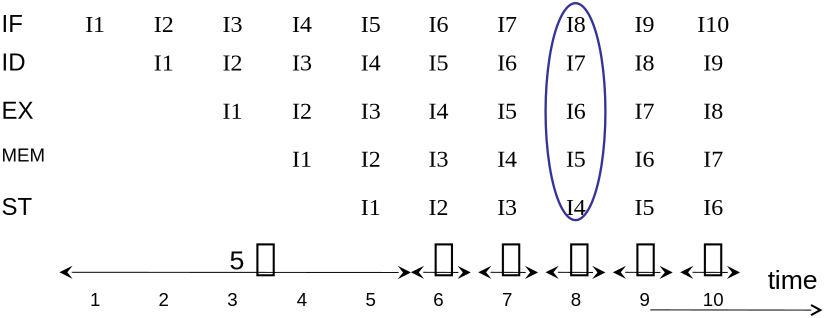
\includegraphics[width=0.9\textwidth]{cpu_pipe_inst_flow-en.pdf}

$\tau = max{\left\lbrace \tau_i \right\rbrace}^k_{i=1}$, where $\tau_i$ is the delay in each stage

The time to execute $n$ instructions in the $k$-stage pipeline
$$T_{k,n} = k \cdot \tau + (n - 1) \tau$$
Speedup
\hskip 7mm
$S_{k,n} = \frac{T_{1,n}}{T_{k,n}} = \frac{n k \tau}{k \tau + (n - 1) \tau}$
\hskip 7mm
$\lim_{n \rightarrow \infty} S_k = k$

\end{frame}

\begin{frame}
\frametitle{Single Cycle Processor (from Lecture 3) -- Datapath}
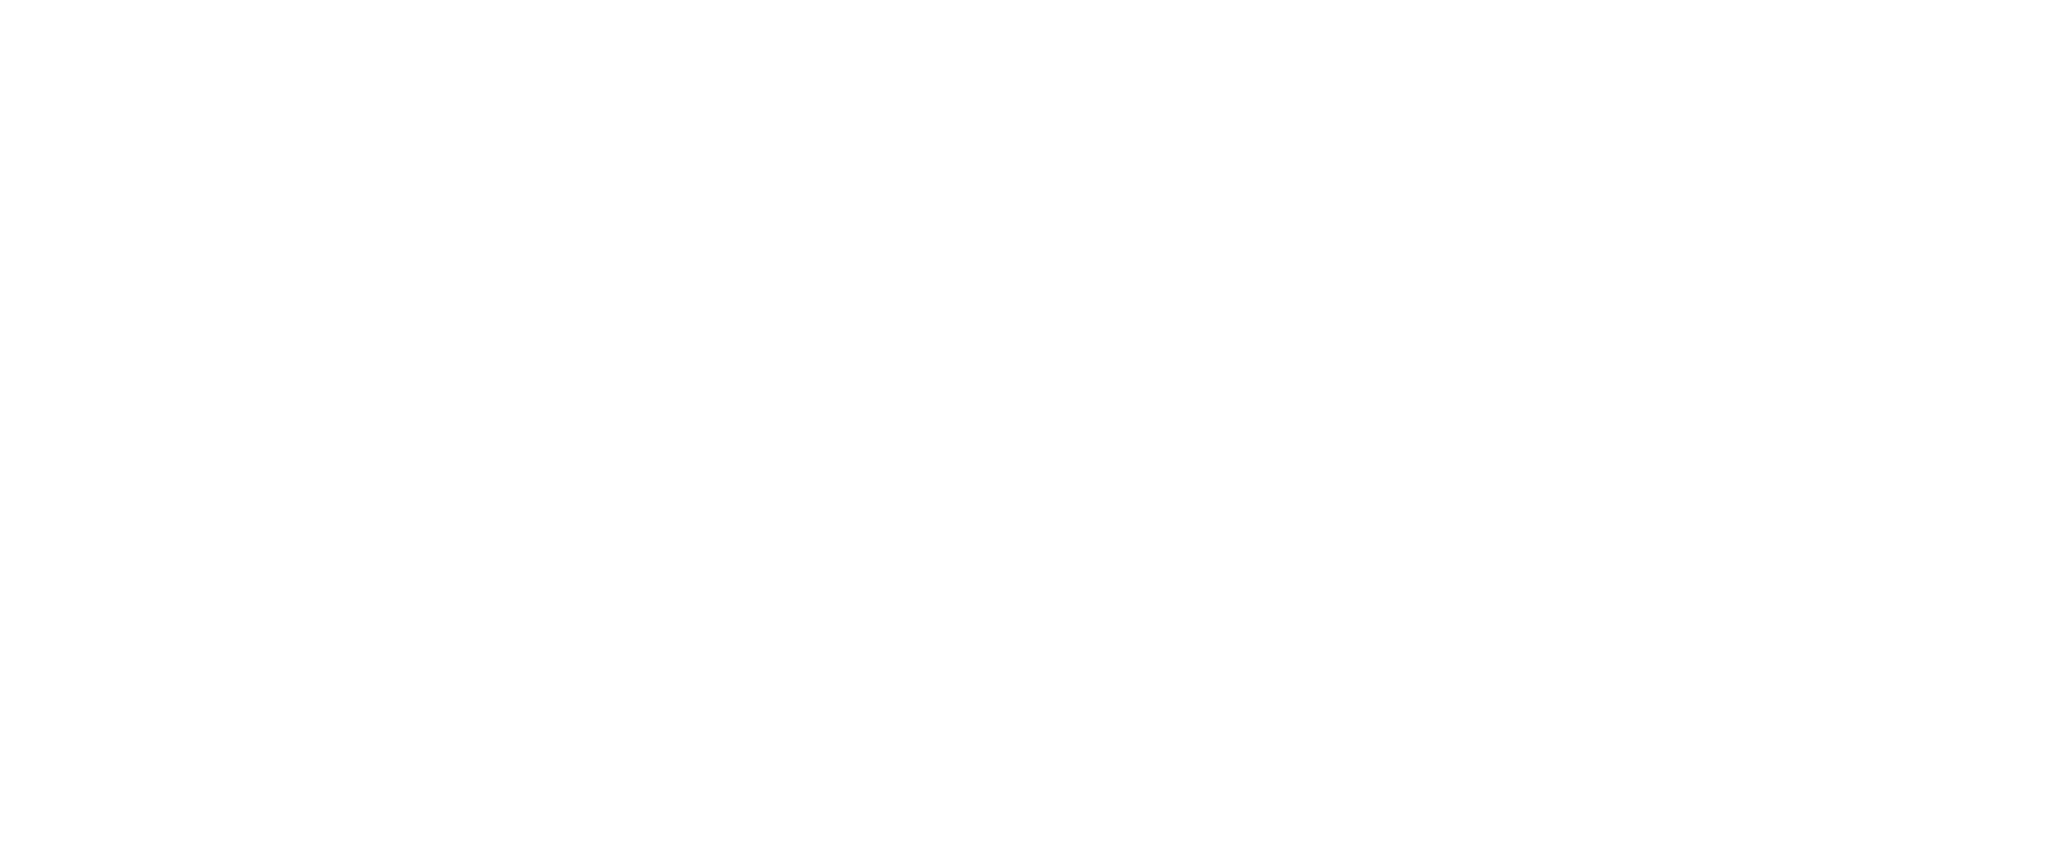
\includegraphics[width=0.95\textwidth]{cpu_nopipe.pdf}
\end{frame}

\begin{frame}
\frametitle{Pipelined Five-Stage Design -- Datapath}
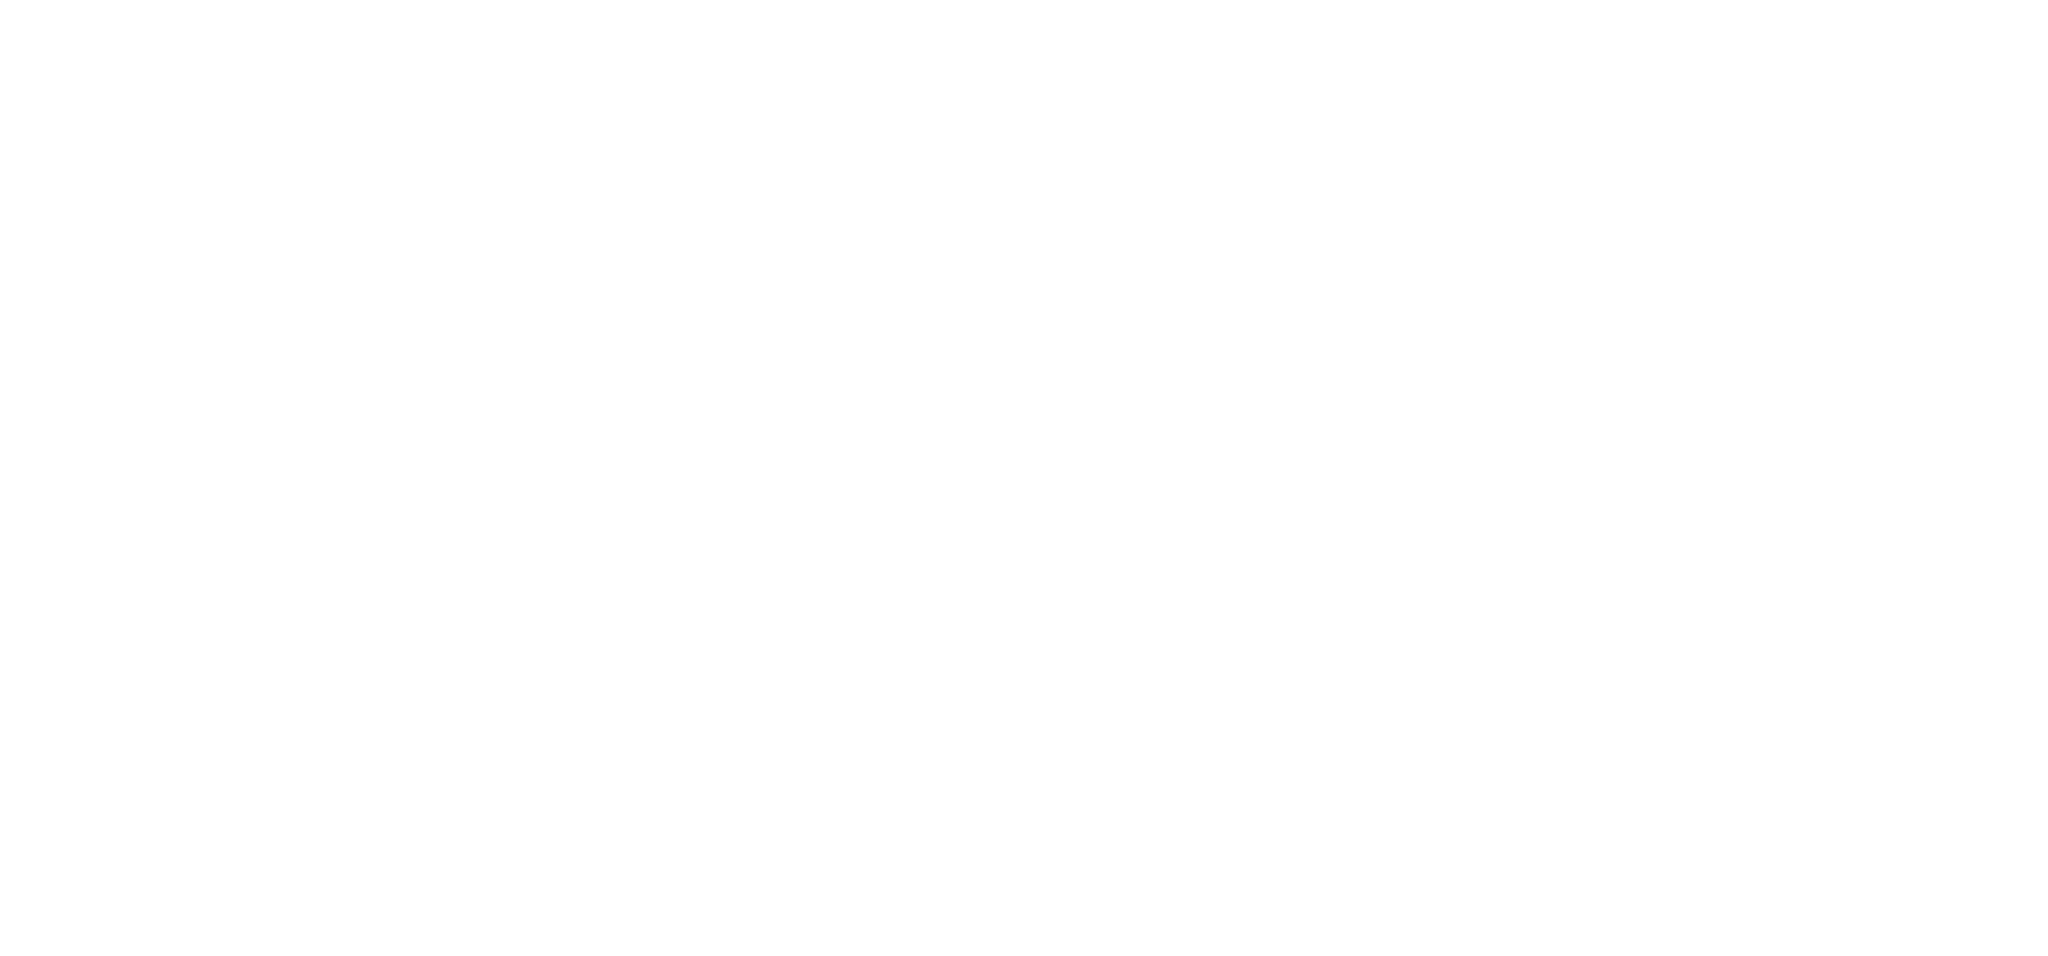
\includegraphics[width=0.95\textwidth]{cpu_pipe.pdf}
\end{frame}

\begin{frame}
\frametitle{Pipelined Five-Stage Design Including Control Unit}
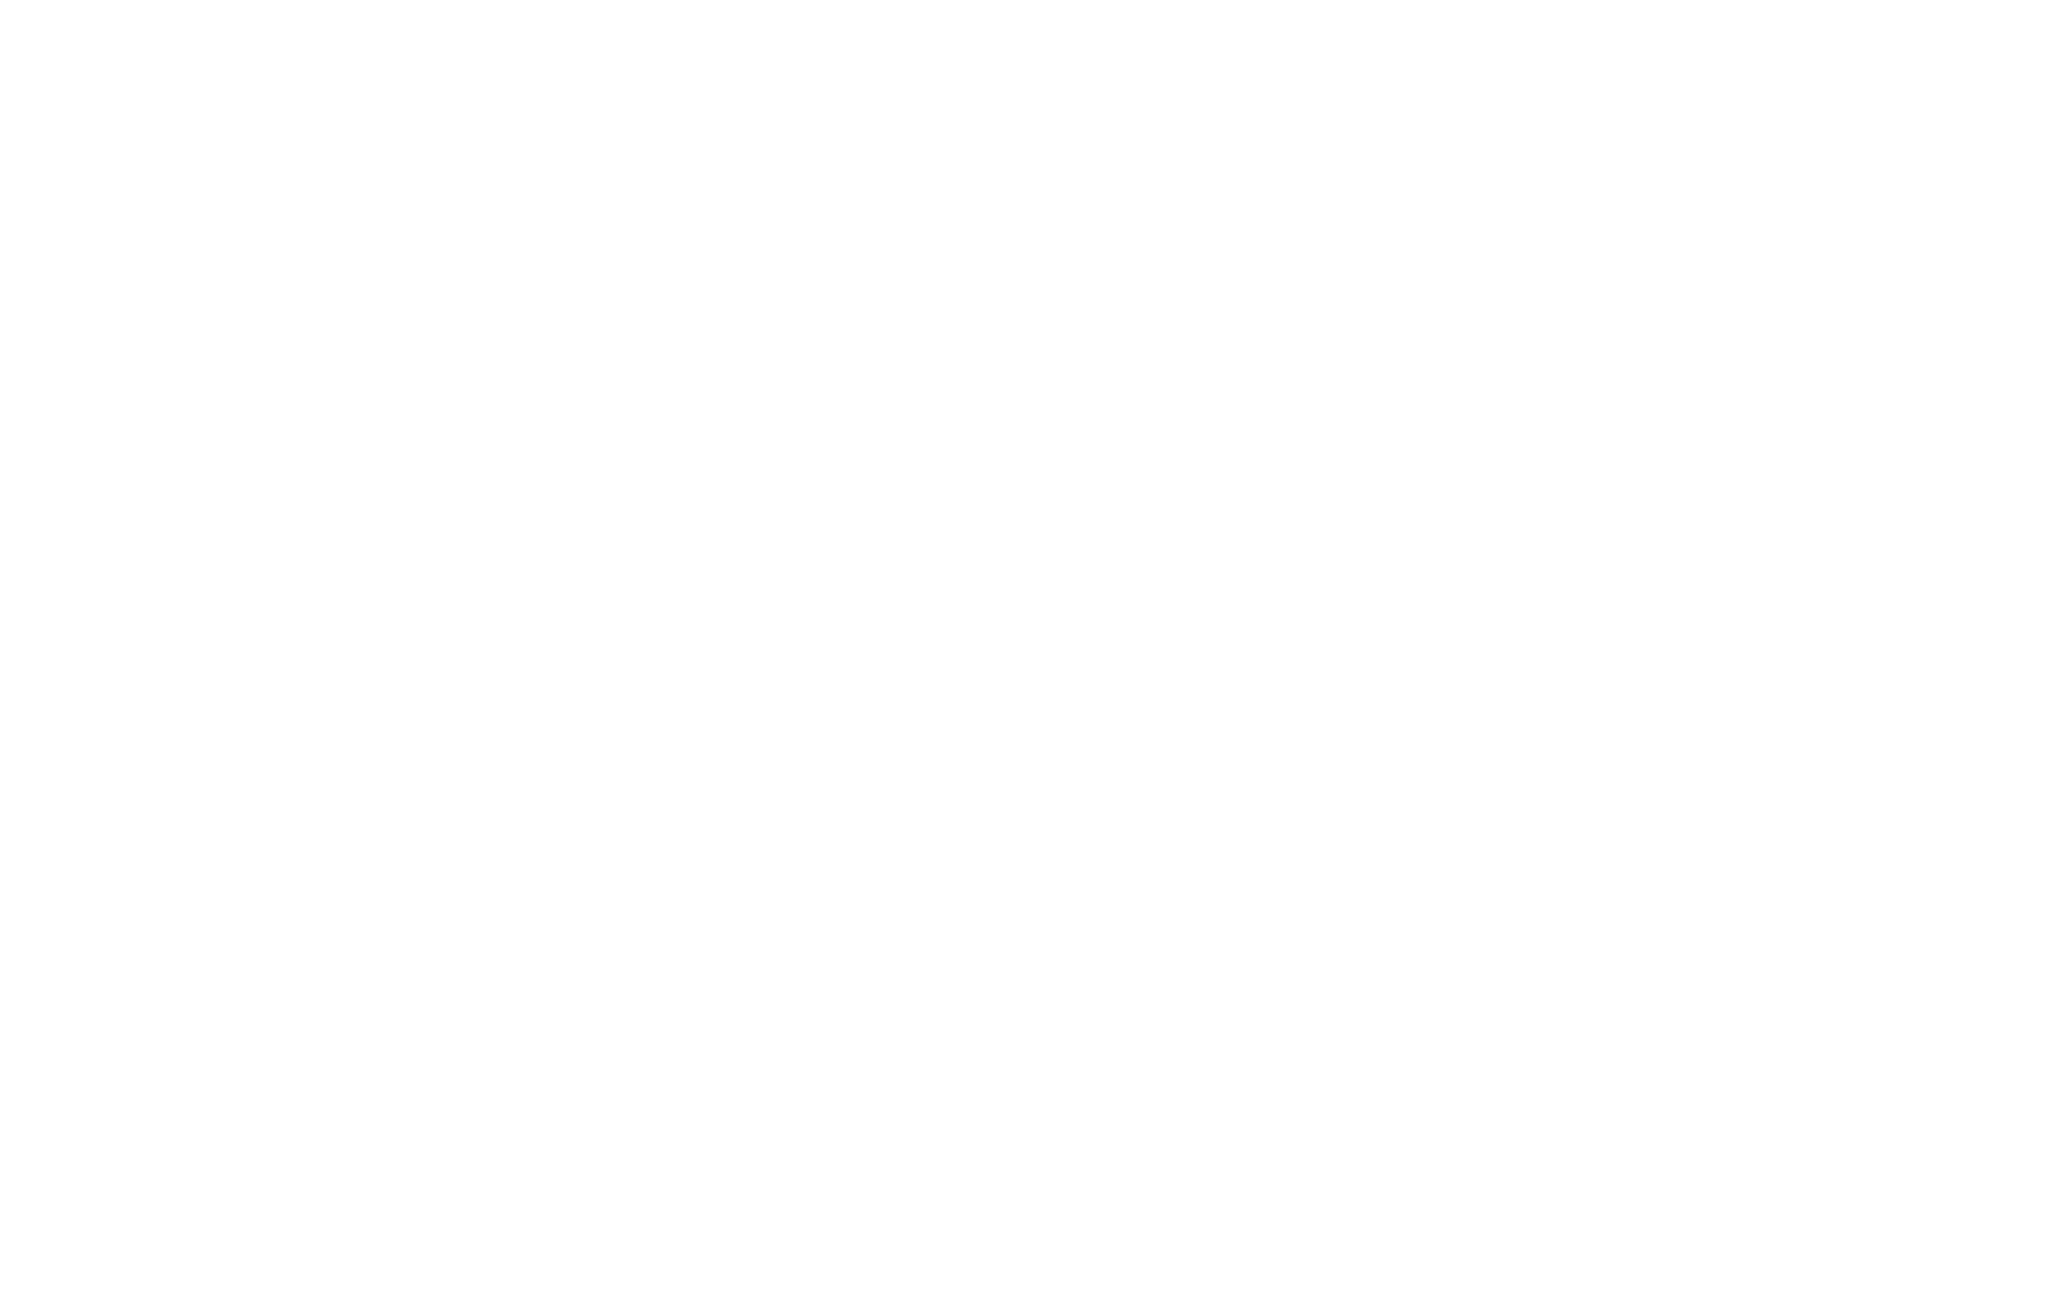
\includegraphics[width=0.95\textwidth]{cpu_ctrl_pipe.pdf}
\end{frame}

\section{Hazard Causes and Theirs Resolution}

\begin{frame}
\frametitle{Semantics Violations -- Data and Control Hazards}
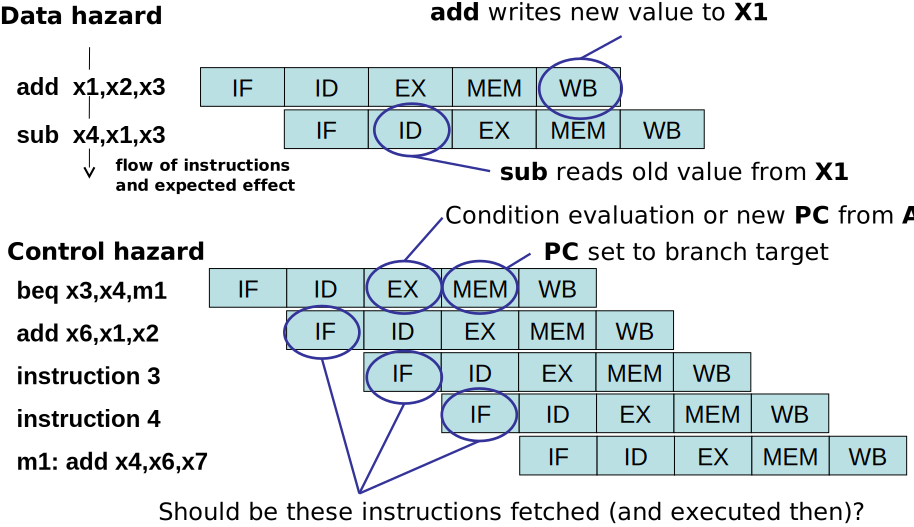
\includegraphics[width=0.95\textwidth]{hazard_kinds-en.pdf}
\end{frame}

\begin{frame}
\frametitle{Cause of Data Hazards}
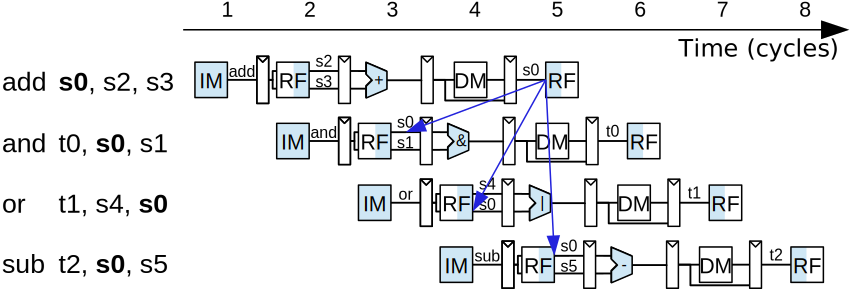
\includegraphics[width=0.95\textwidth]{hazard_data-en.pdf}

\vskip 2 mm

\begin{itemize}
 \item The register file is accessed from two stages (Decode, WriteBack) --
       writing is done in the first half of the cycle, reading in the second half $\Rightarrow$ there is no hazard for sub \textbf{s0} input operand
 \item Read-After-Write (RAW) hazard occurs in instructions
       \textbf{and} and \textbf{or} when reading \textbf{s0} in cycle 3 and 4
 \item How can such hazard be prevented without pipeline throughput degradation?
\end{itemize}

\end{frame}


\begin{frame}
\frametitle{Data Hazard in the "and" Instruction in the QtRVSim}
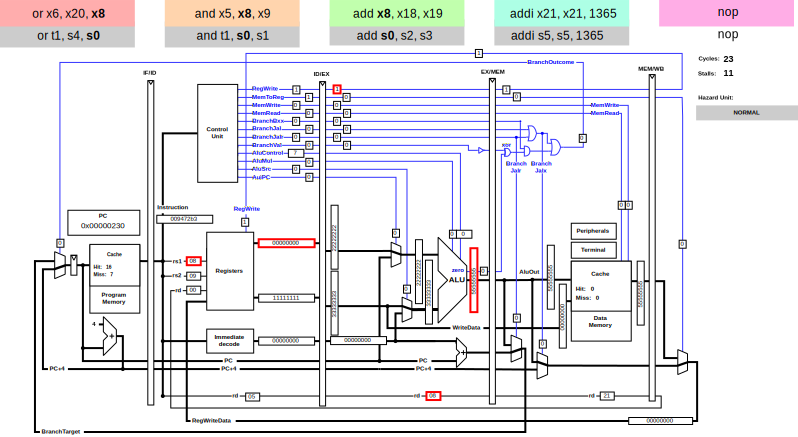
\includegraphics[width=0.95\textwidth]{hazard_qtrvsim.pdf}

{\tiny
QtRvSim \url{https://github.com/cvut/qtrvsim}
}

{\Tiny
\url{https://gitlab.fel.cvut.cz/b35apo/stud-support/-/blob/master/seminaries/qtrvsim/hazards-from-lecture/alu-hazards.S}
}

\end{frame}

\begin{frame}
\frametitle{QtRVSim -- Resolve Data Hazard by Stall}
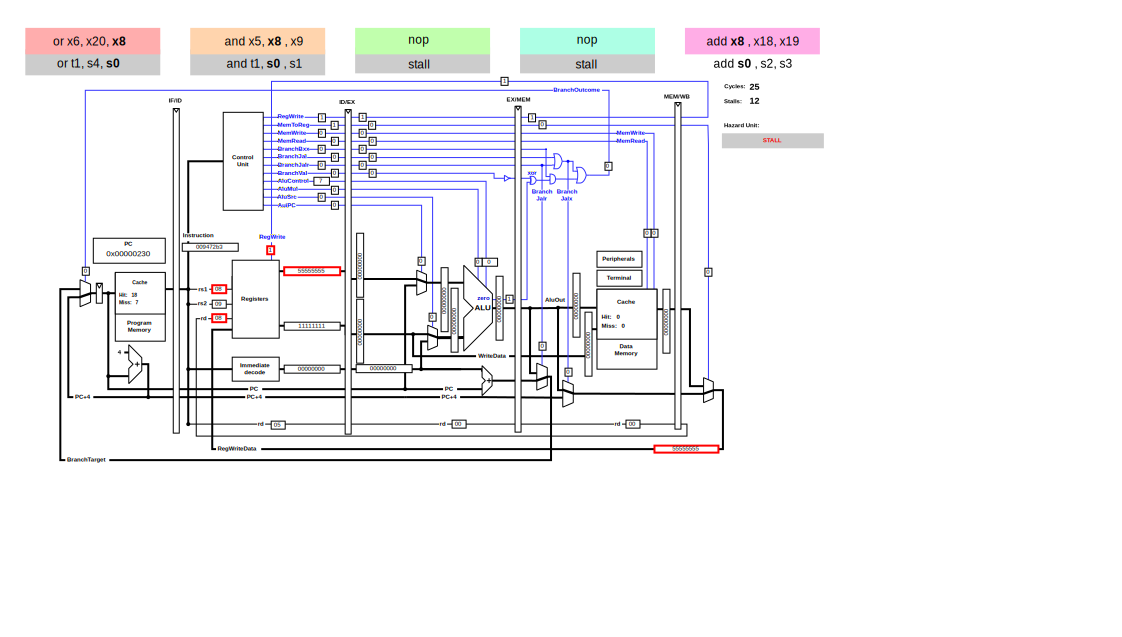
\includegraphics[width=0.95\textwidth]{hazard_stall_qtrvsim.pdf}

{\tiny
QtRvSim \url{https://github.com/cvut/qtrvsim}
}

{\Tiny
\url{https://gitlab.fel.cvut.cz/b35apo/stud-support/-/blob/master/seminaries/qtrvsim/hazards-from-lecture/alu-hazards.S}
}

\end{frame}


\begin{frame}
\frametitle{Data Hazard Resolution by Forwarding}
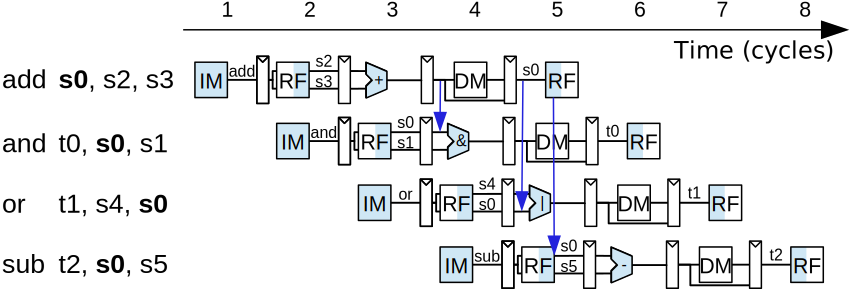
\includegraphics[width=0.85\textwidth]{forward_data-en.pdf}

\begin{itemize}
 \item If a result is available (computed) before subsequent instruction(s) requires the value then data hazard can be avoided by forwarding
 \item Data hazard occurs in the considered pipeline design if a source register
       (\textbf{rs1}, \textbf{rs2}) in the \textbf{EX} stage corresponds to the target register
       in \textbf{MEM} or \textbf{WB} (except X0/zero)
 \item The register numbers are fed to the Hazard Unit (HU)
\end{itemize}

\end{frame}

\begin{frame}
\frametitle{Recap of Previous Design and Prepare It for Forwarding}
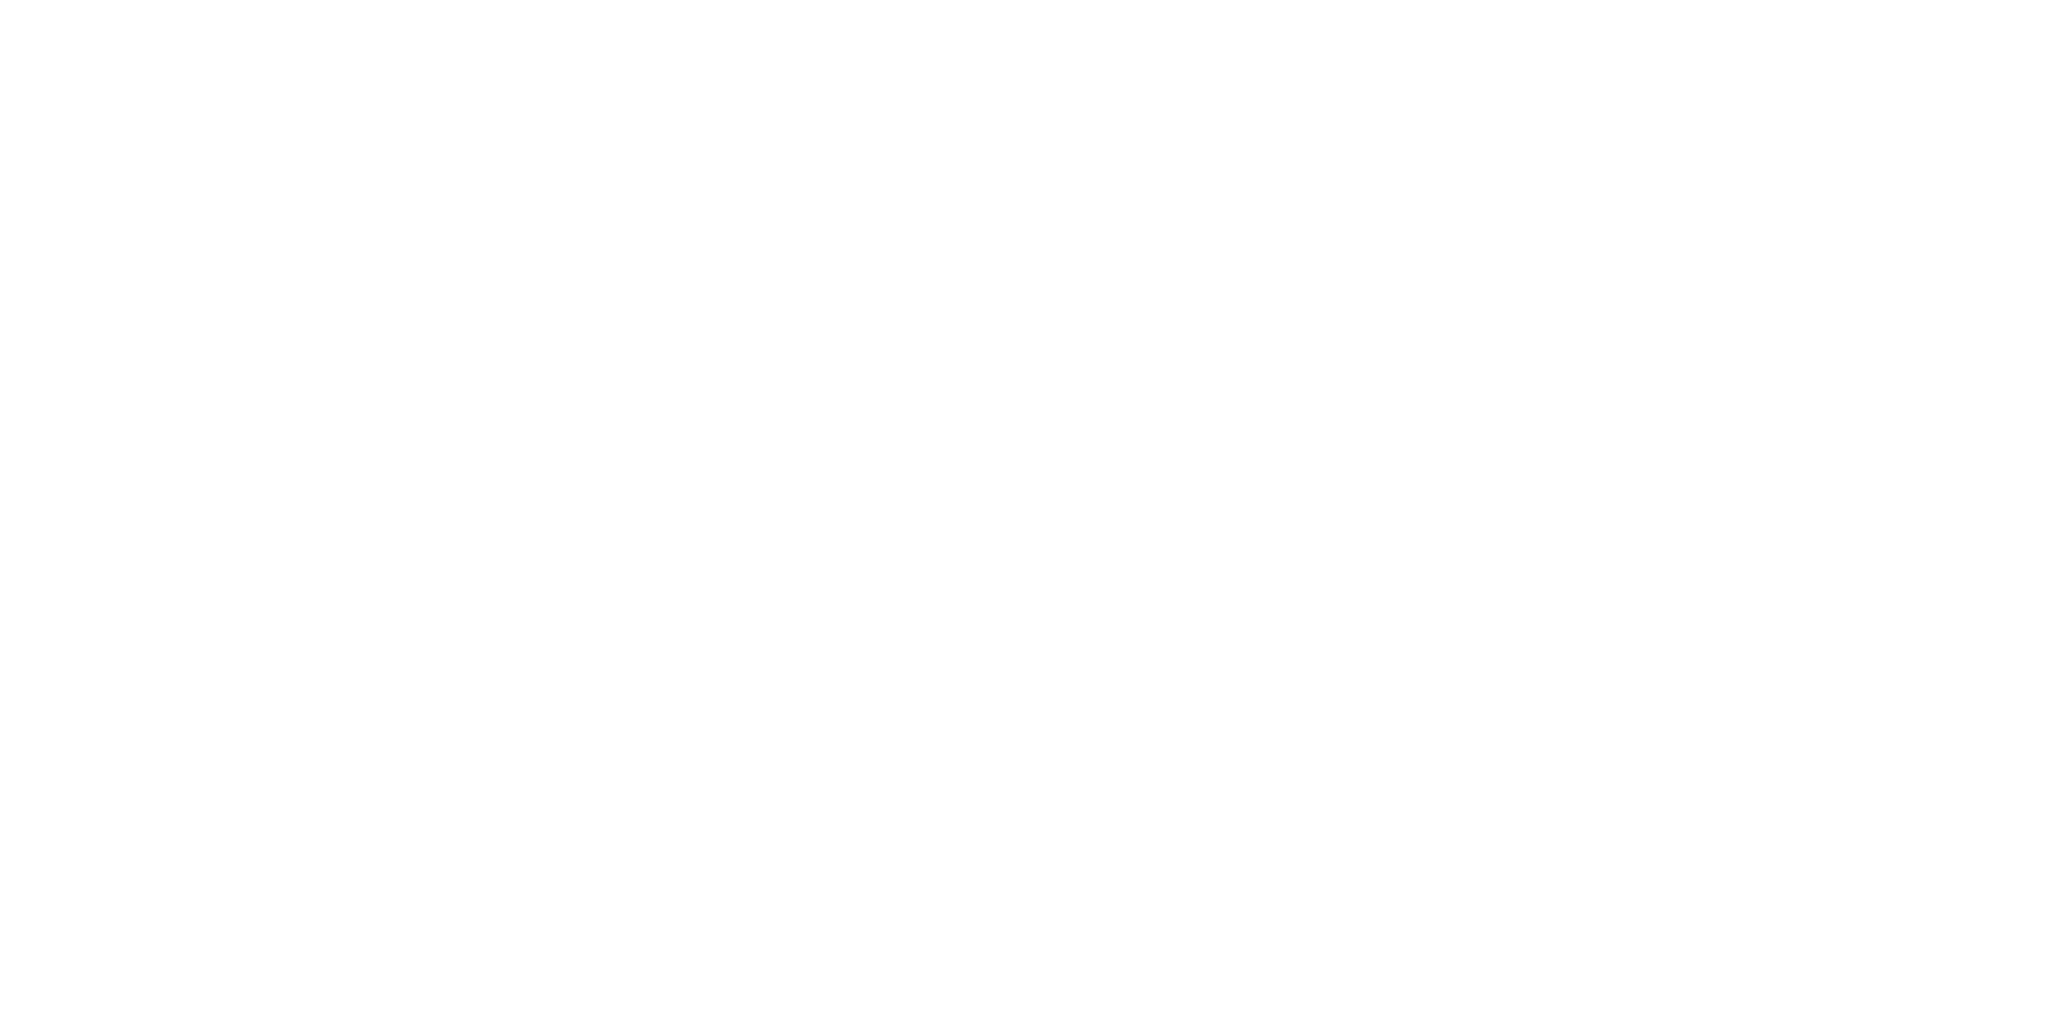
\includegraphics[width=0.95\textwidth]{noforward_data.pdf}

You need to know the previous \textbf{A1} (\textbf{rs1}) and \textbf{A2} (\textbf{rs2}) in \textbf{EX}.
The \textbf{RegWrite} signals from \textbf{MEM} and \textbf{WB} has to be monitored as well to check
that the register specified by \textbf{WriteReg} in \textbf{MEM} and \textbf{WB} is indeed being written.

\end{frame}

\begin{frame}
\frametitle{Processor Design with MEM and WB to EX Forwarding}
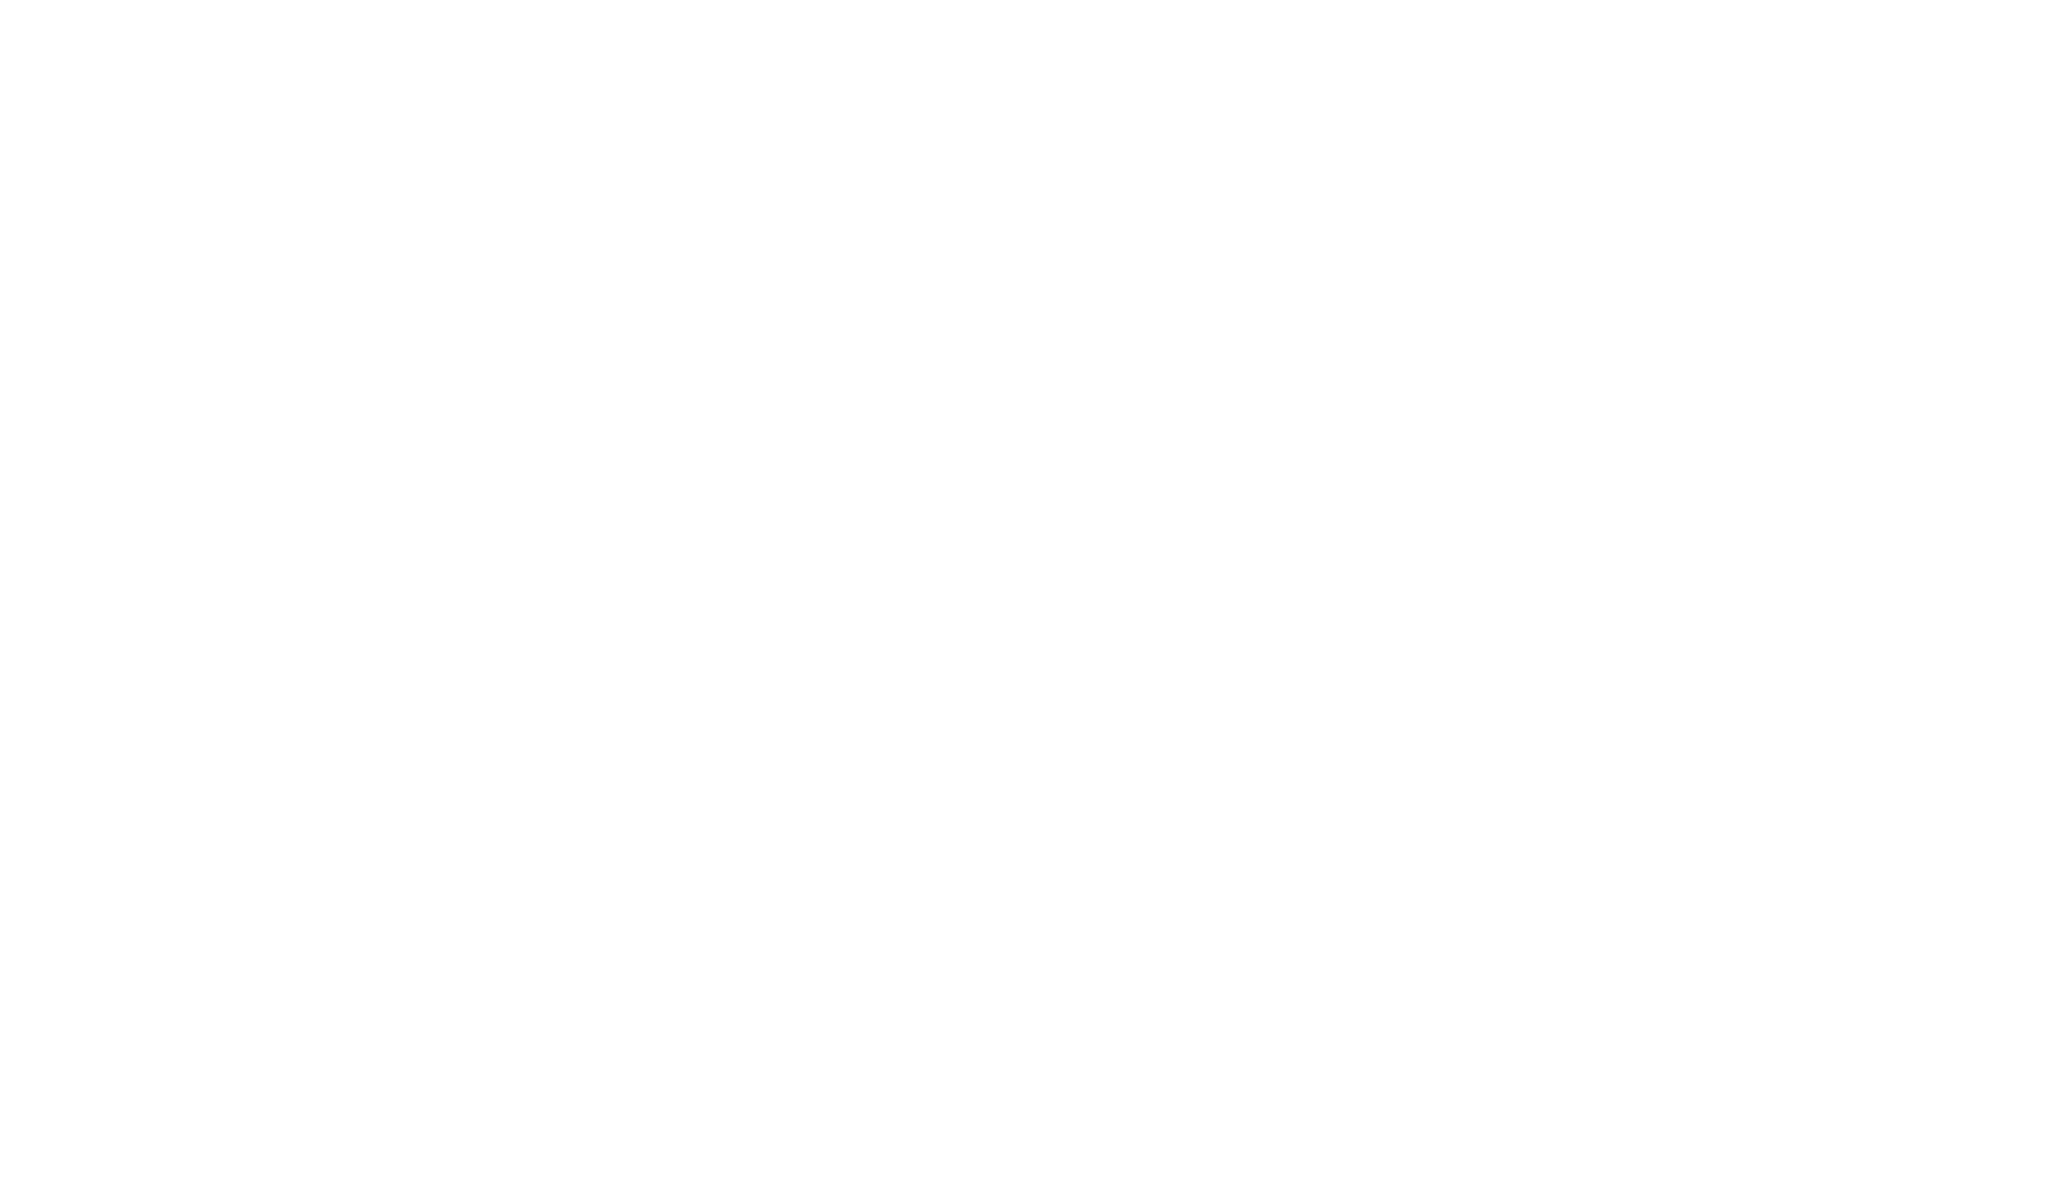
\includegraphics[width=0.95\textwidth]{forward_hazard.pdf}
\end{frame}

\begin{frame}
\frametitle{QtRvSim -- Data Hazards Resolved by Forwarding}
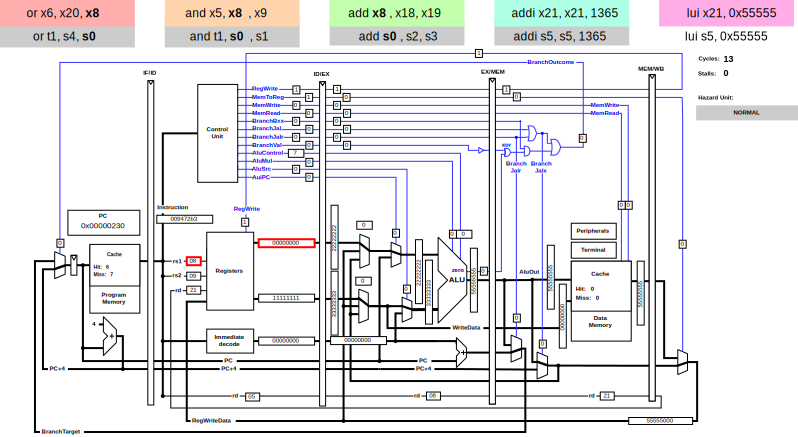
\includegraphics[width=0.95\textwidth]{hazard_forwarding.pdf}

{\tiny
QtRvSim \url{https://github.com/cvut/qtrvsim}
}

{\Tiny
\url{https://gitlab.fel.cvut.cz/b35apo/stud-support/-/blob/master/seminaries/qtrvsim/hazards-from-lecture/alu-hazards.S}
}

\end{frame}

\begin{frame}
\frametitle{Forwarding the "and" Instruction rs1 Input from MEM}
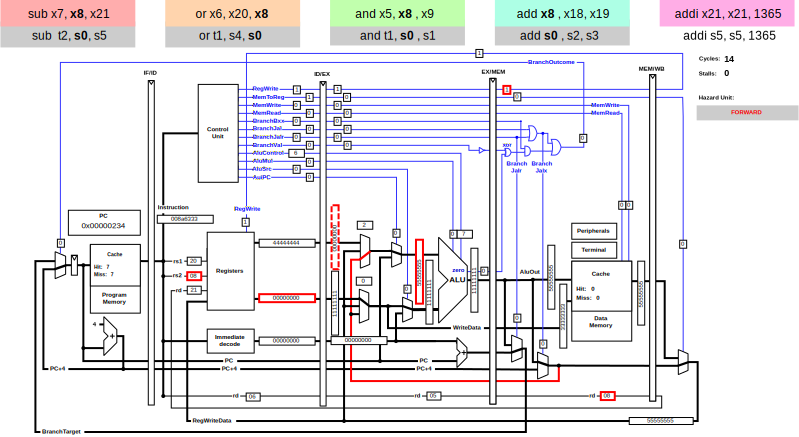
\includegraphics[width=0.95\textwidth]{hazard_forwarding2.pdf}

{\tiny
QtRvSim \url{https://github.com/cvut/qtrvsim}
}

{\Tiny
\url{https://gitlab.fel.cvut.cz/b35apo/stud-support/-/blob/master/seminaries/qtrvsim/hazards-from-lecture/alu-hazards.S}
}

\end{frame}

\begin{frame}
\frametitle{Forwarding the "or" Instruction rs2 Input from WB}
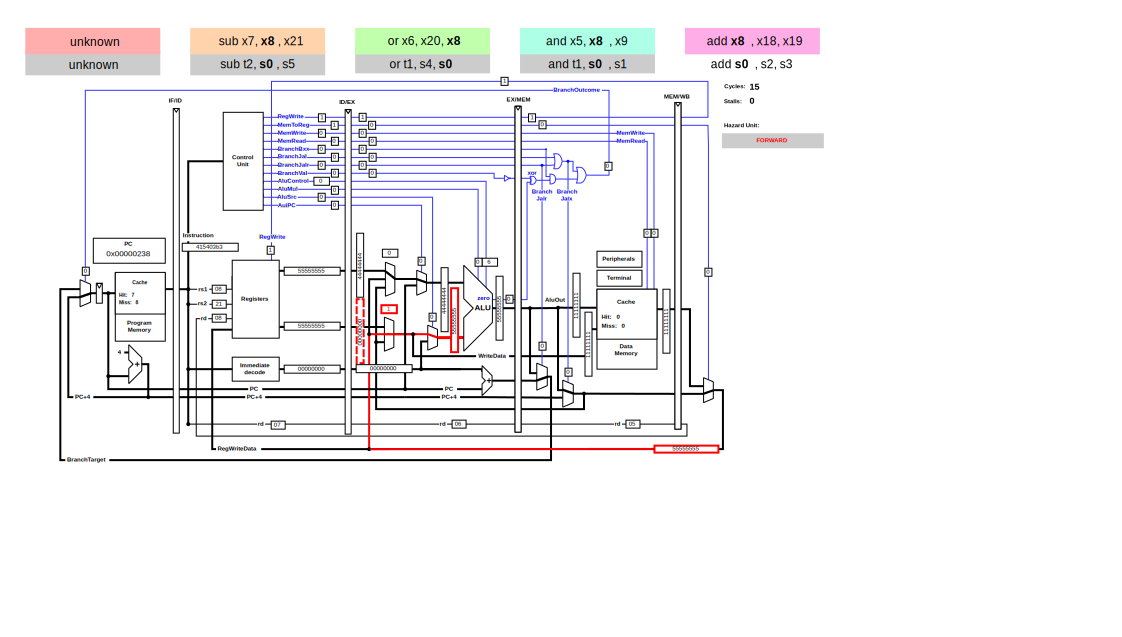
\includegraphics[width=0.95\textwidth]{hazard_forwarding3.pdf}

{\tiny
QtRvSim \url{https://github.com/cvut/qtrvsim}
}

{\Tiny
\url{https://gitlab.fel.cvut.cz/b35apo/stud-support/-/blob/master/seminaries/qtrvsim/hazards-from-lecture/alu-hazards.S}
}

\end{frame}

\begin{frame}
\frametitle{Persisting Problem in the "lw" Case -- Solved by Stalling}
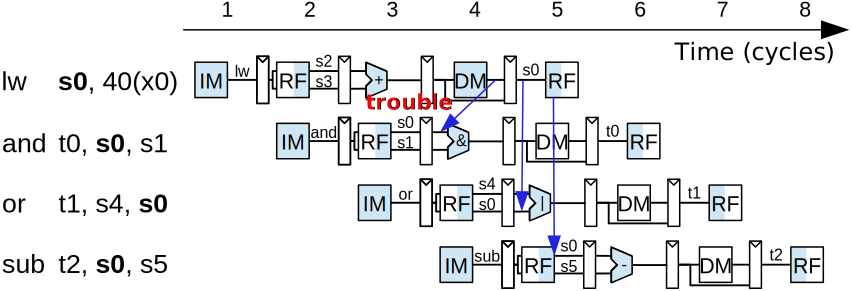
\includegraphics[width=0.85\textwidth]{pipeline_stall-en.pdf}

\begin{itemize}
 \item If subsequent instructions require result before it is available in CPU then the pipeline has to be stalled (\textbf{stall} and \textbf{nop} inserted/interstage flush)
 \item Stalling resolves hazards but degrades throughput
 \item Stages preceding the stage affected by the hazard are suspended until all results required by subsequent instructions are available then results are forwarded to all locations which required their values
\end{itemize}

\end{frame}

\begin{frame}
\frametitle{Data Hazard Resolution by Stalling}
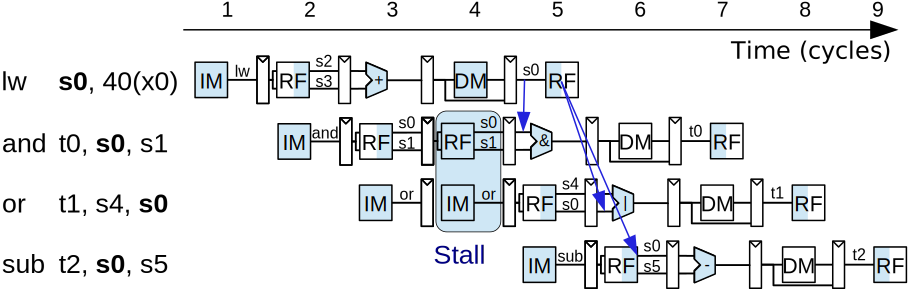
\includegraphics[width=0.85\textwidth]{pipeline_stall2-en.pdf}

\begin{itemize}
 \item Stalling is realized by holding the contents of the interstage registers
       (by gating their clock or blocking their latch enable signals)
 \item Results from stage(s) with missing data/dependencies are discarded, coresponding instruction(s) memory and register write enable as well as other signals are reset (held inactive)
 \item Both is achieved by introduction of control signals to hold and/or reset inter-stages registers
\end{itemize}

\end{frame}

\begin{frame}
\frametitle{Avoid Remaining Data Hazards by Stalling -- CPU Diagram}
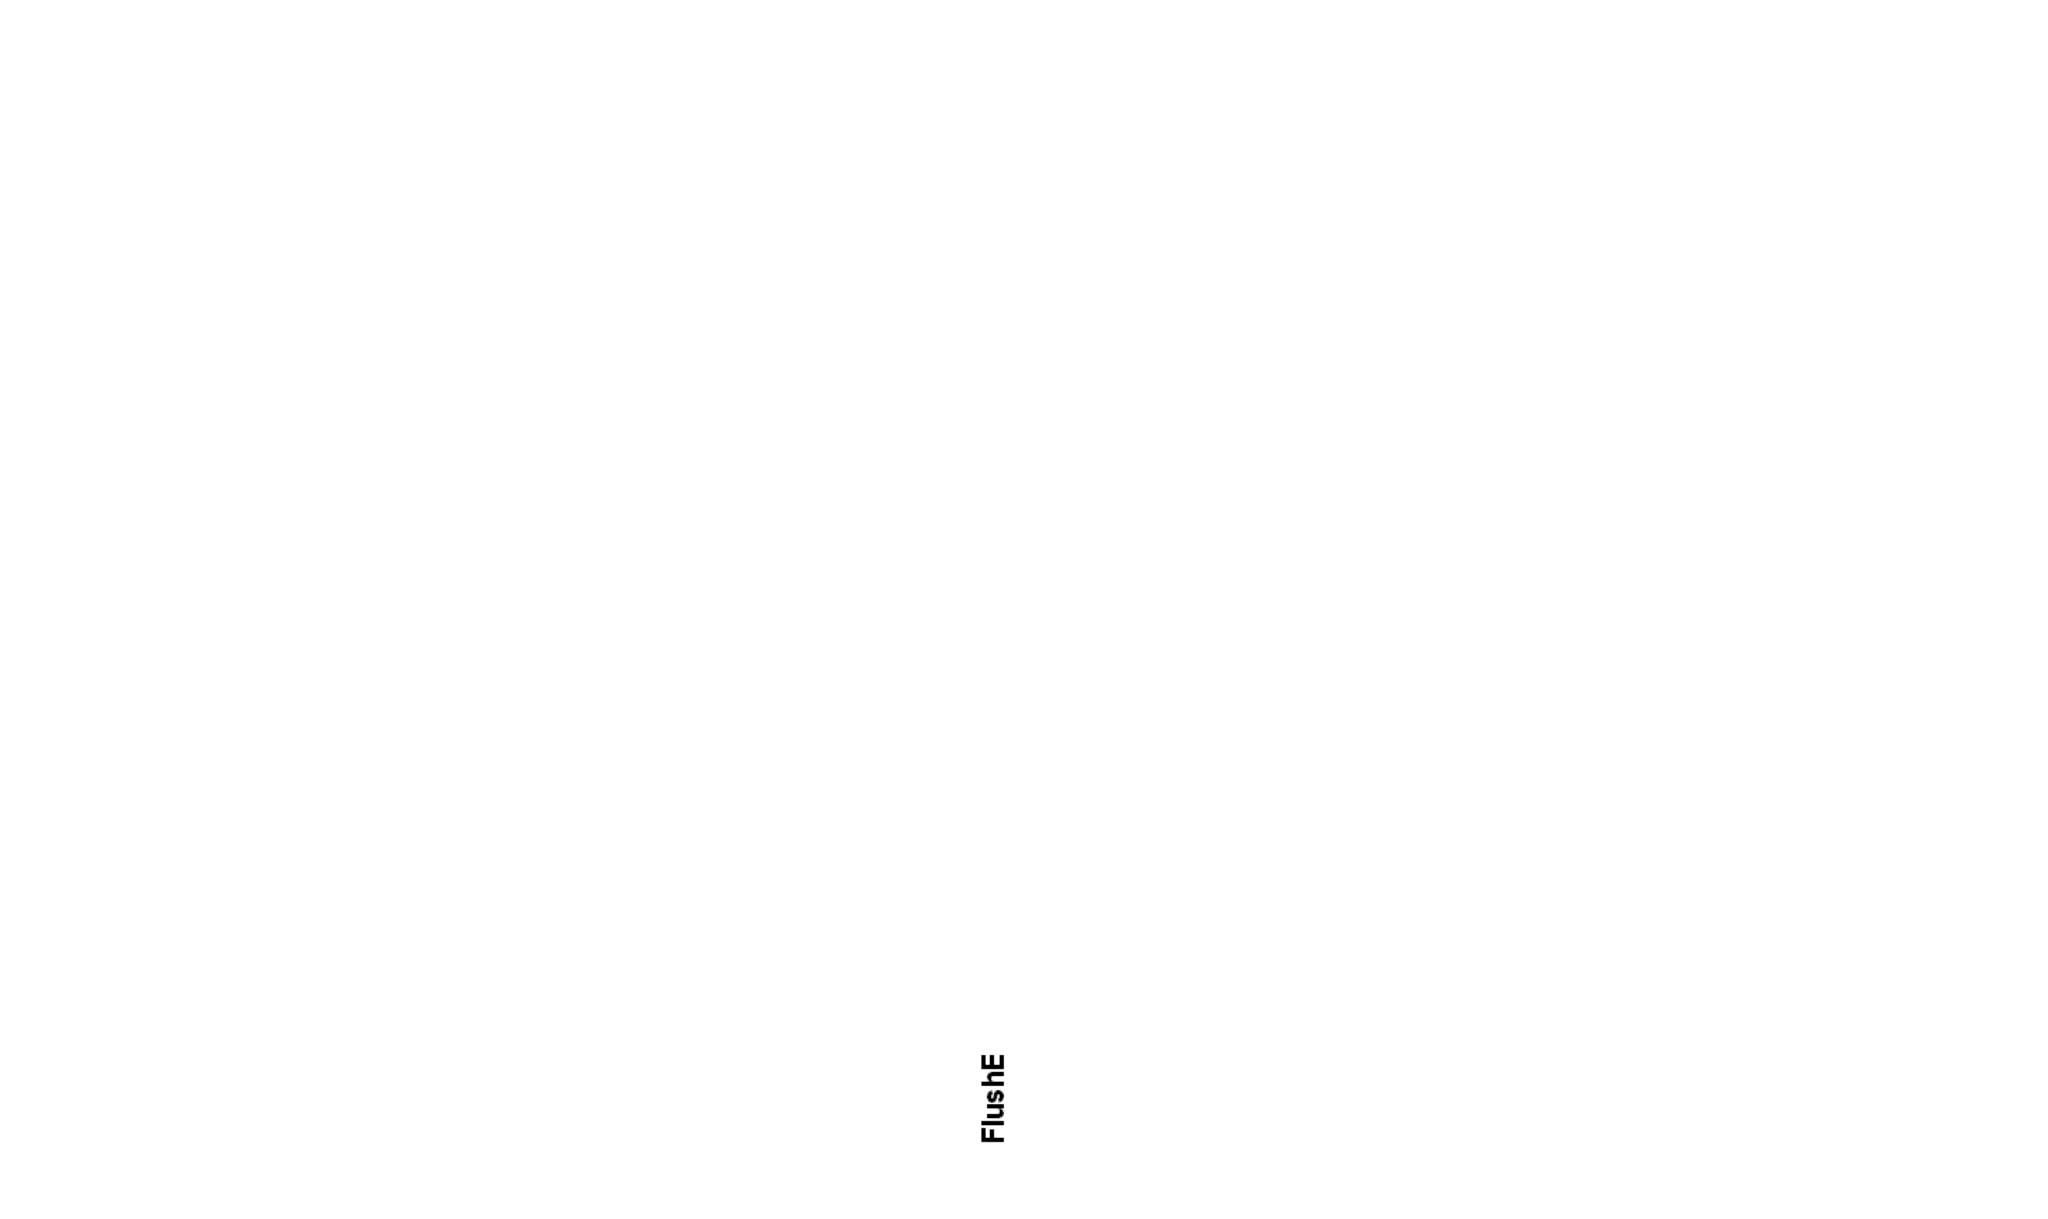
\includegraphics[width=0.95\textwidth]{cpu_fwd_stall.pdf}
\end{frame}

\begin{frame}
\frametitle{QtRvSim -- Data Hazard in "lw" Avoided by Stalling}
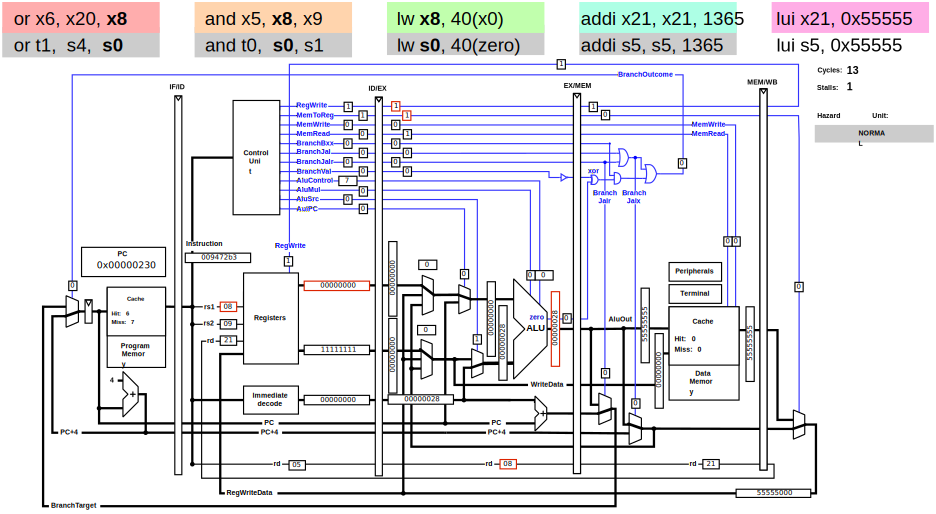
\includegraphics[width=0.95\textwidth]{hazard_stall_qtrvsim2.pdf}
{\tiny
QtRvSim \url{https://github.com/cvut/qtrvsim}
}

{\Tiny
\url{https://gitlab.fel.cvut.cz/b35apo/stud-support/-/blob/master/seminaries/qtrvsim/hazards-from-lecture/lw-hazards.S}
}

\end{frame}

\begin{frame}
\frametitle{QtRvSim -- Data Hazard in "lw" Avoided by Stalling}
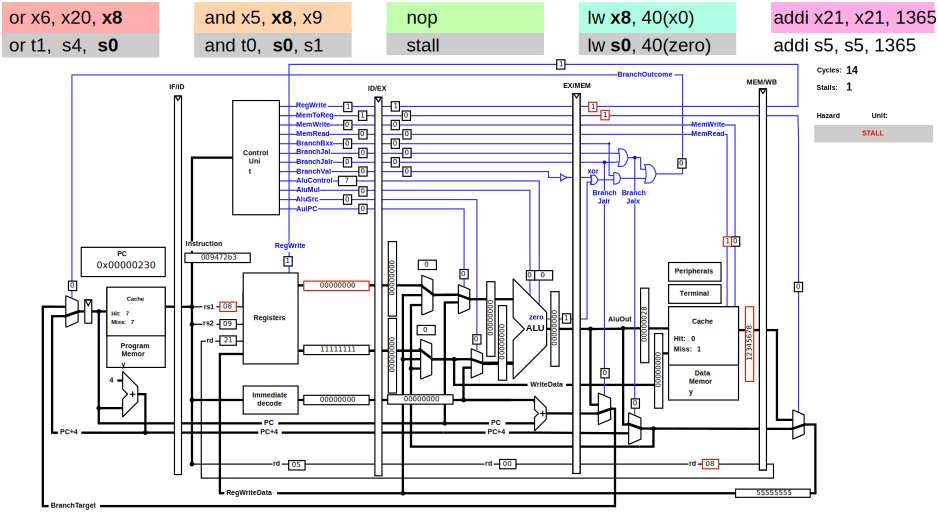
\includegraphics[width=0.95\textwidth]{hazard_stall_qtrvsim3.pdf}

{\tiny
QtRvSim \url{https://github.com/cvut/qtrvsim}
}

{\Tiny
\url{https://gitlab.fel.cvut.cz/b35apo/stud-support/-/blob/master/seminaries/qtrvsim/hazards-from-lecture/lw-hazards.S}
}

\end{frame}

\begin{frame}
\frametitle{QtRvSim -- Data Hazard in "lw" Avoided by Stalling}
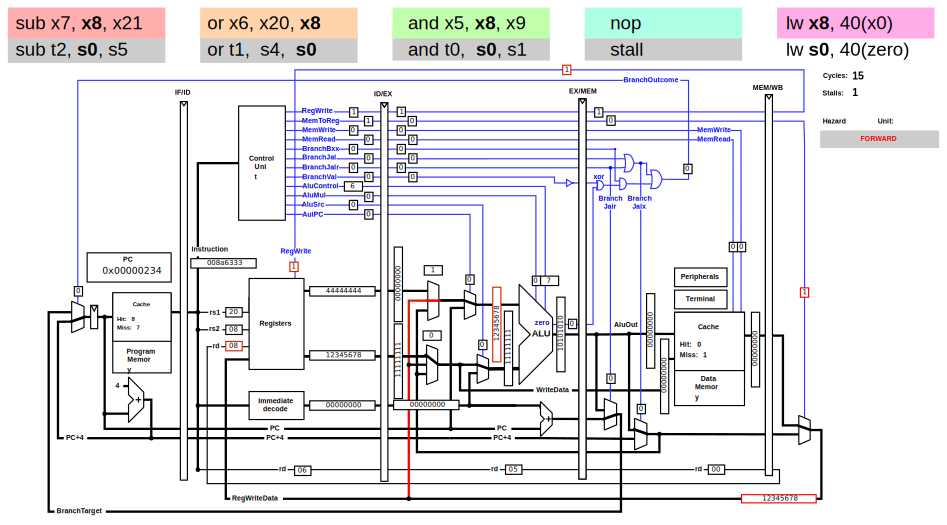
\includegraphics[width=0.95\textwidth]{hazard_stall_qtrvsim4.pdf}

{\tiny
QtRvSim \url{https://github.com/cvut/qtrvsim}
}

{\Tiny
\url{https://gitlab.fel.cvut.cz/b35apo/stud-support/-/blob/master/seminaries/qtrvsim/hazards-from-lecture/lw-hazards.S}
}

\end{frame}

\section{Control Hazards}

\begin{frame}
\frametitle{Control Hazards (Branch and Jump Instructions)}
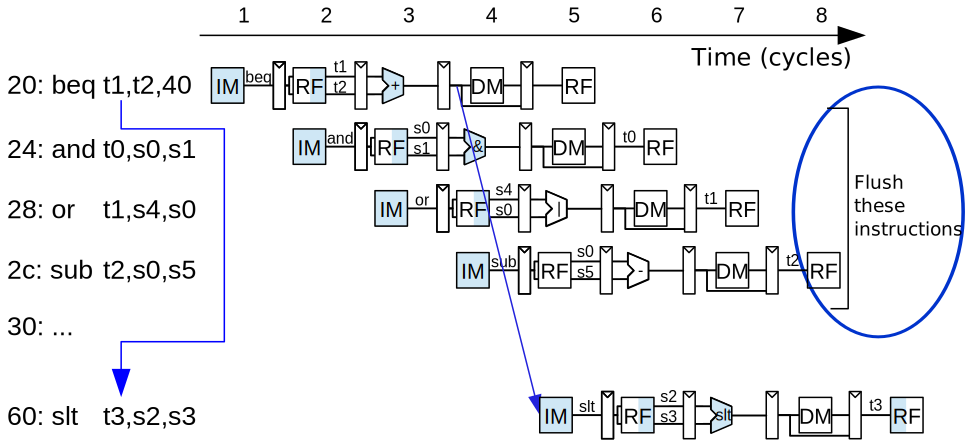
\includegraphics[width=0.85\textwidth]{hazard_ctrl-en.pdf}

\begin{itemize}
 \item The result is not known until the fourth cycle, then it is loaded to the PC
       and so the first instruction at the jump target address may not be loaded until cycle five.
 \item Jumps in this way represent a major limitation on the time usage of the execution units in the pipeline
\end{itemize}

\end{frame}

\begin{frame}
\frametitle{Alternative, Move Branch Decision Earlier}
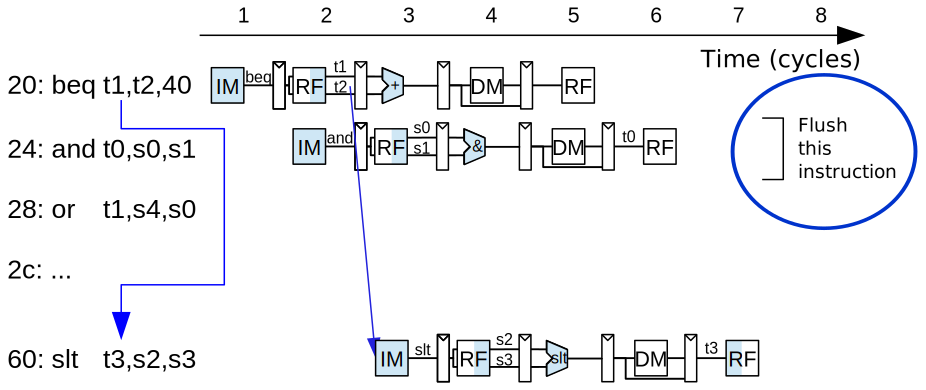
\includegraphics[width=0.85\textwidth]{hazard_ctrl2-en.pdf}

\begin{itemize}
 \item This causes structural hazard, \textbf{ALU} is needed in both \textbf{EX} and \textbf{ID}.
 \item Structural hazards can be solved by duplicating given component (ALU in the respective case). A complete adder, subtractor or comparison
       takes a long time, a solution may be to restrict the branch conditions to equality/non-equality only (just xor
       between operands led to bitwise nor)
\end{itemize}

\end{frame}

\begin{frame}
\frametitle{MIPS Resolve Control Hazards by Early Evaluate and Flush}
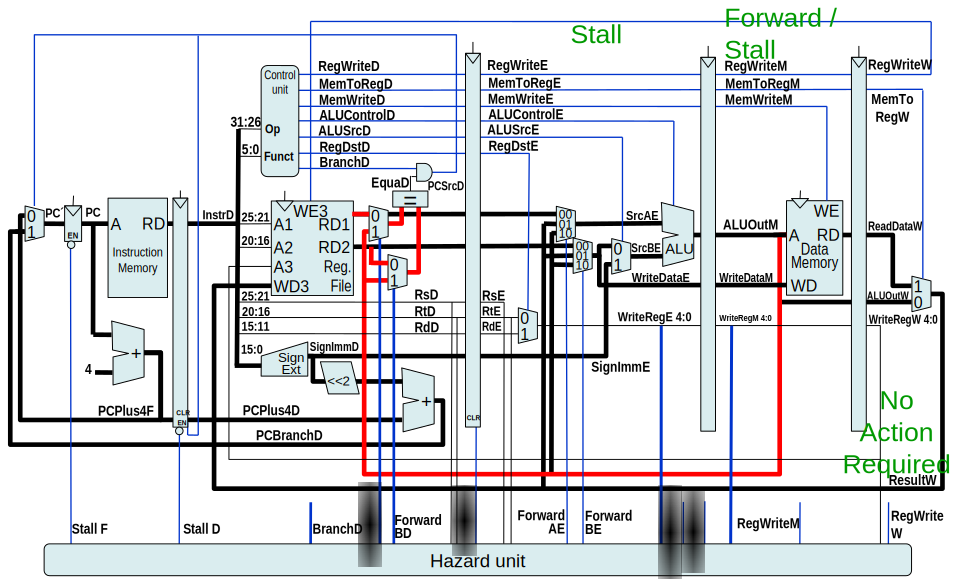
\includegraphics[width=0.90\textwidth]{hazard_ctrl_mips2.pdf}
\end{frame}

\begin{frame}
\frametitle{Resolution of Hazards on Comparator Inputs -- MIPS}
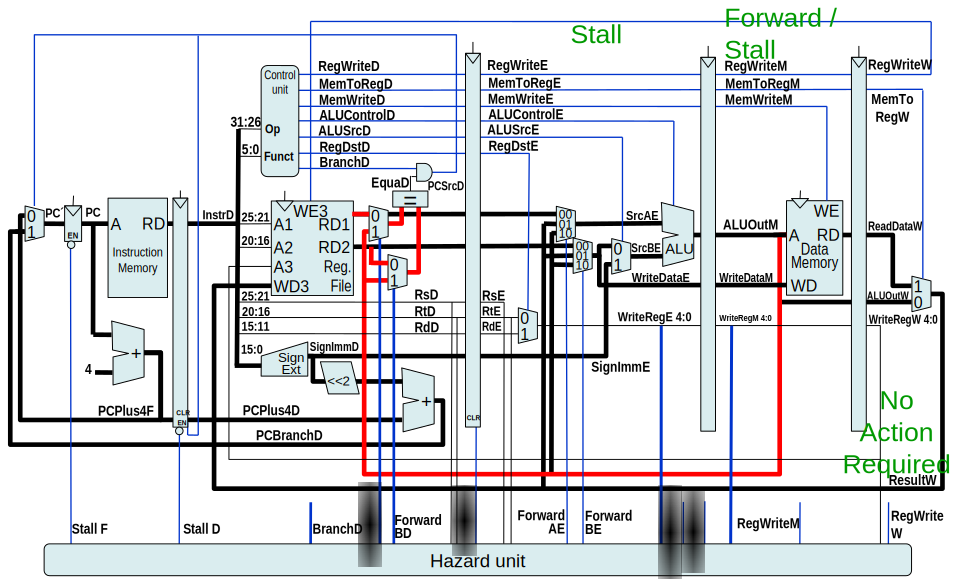
\includegraphics[width=0.90\textwidth]{hazard_ctrl_mips2.pdf}
\end{frame}

\begin{frame}
\frametitle{Branch Prediction and Speculative Execution (Next Lect.)}
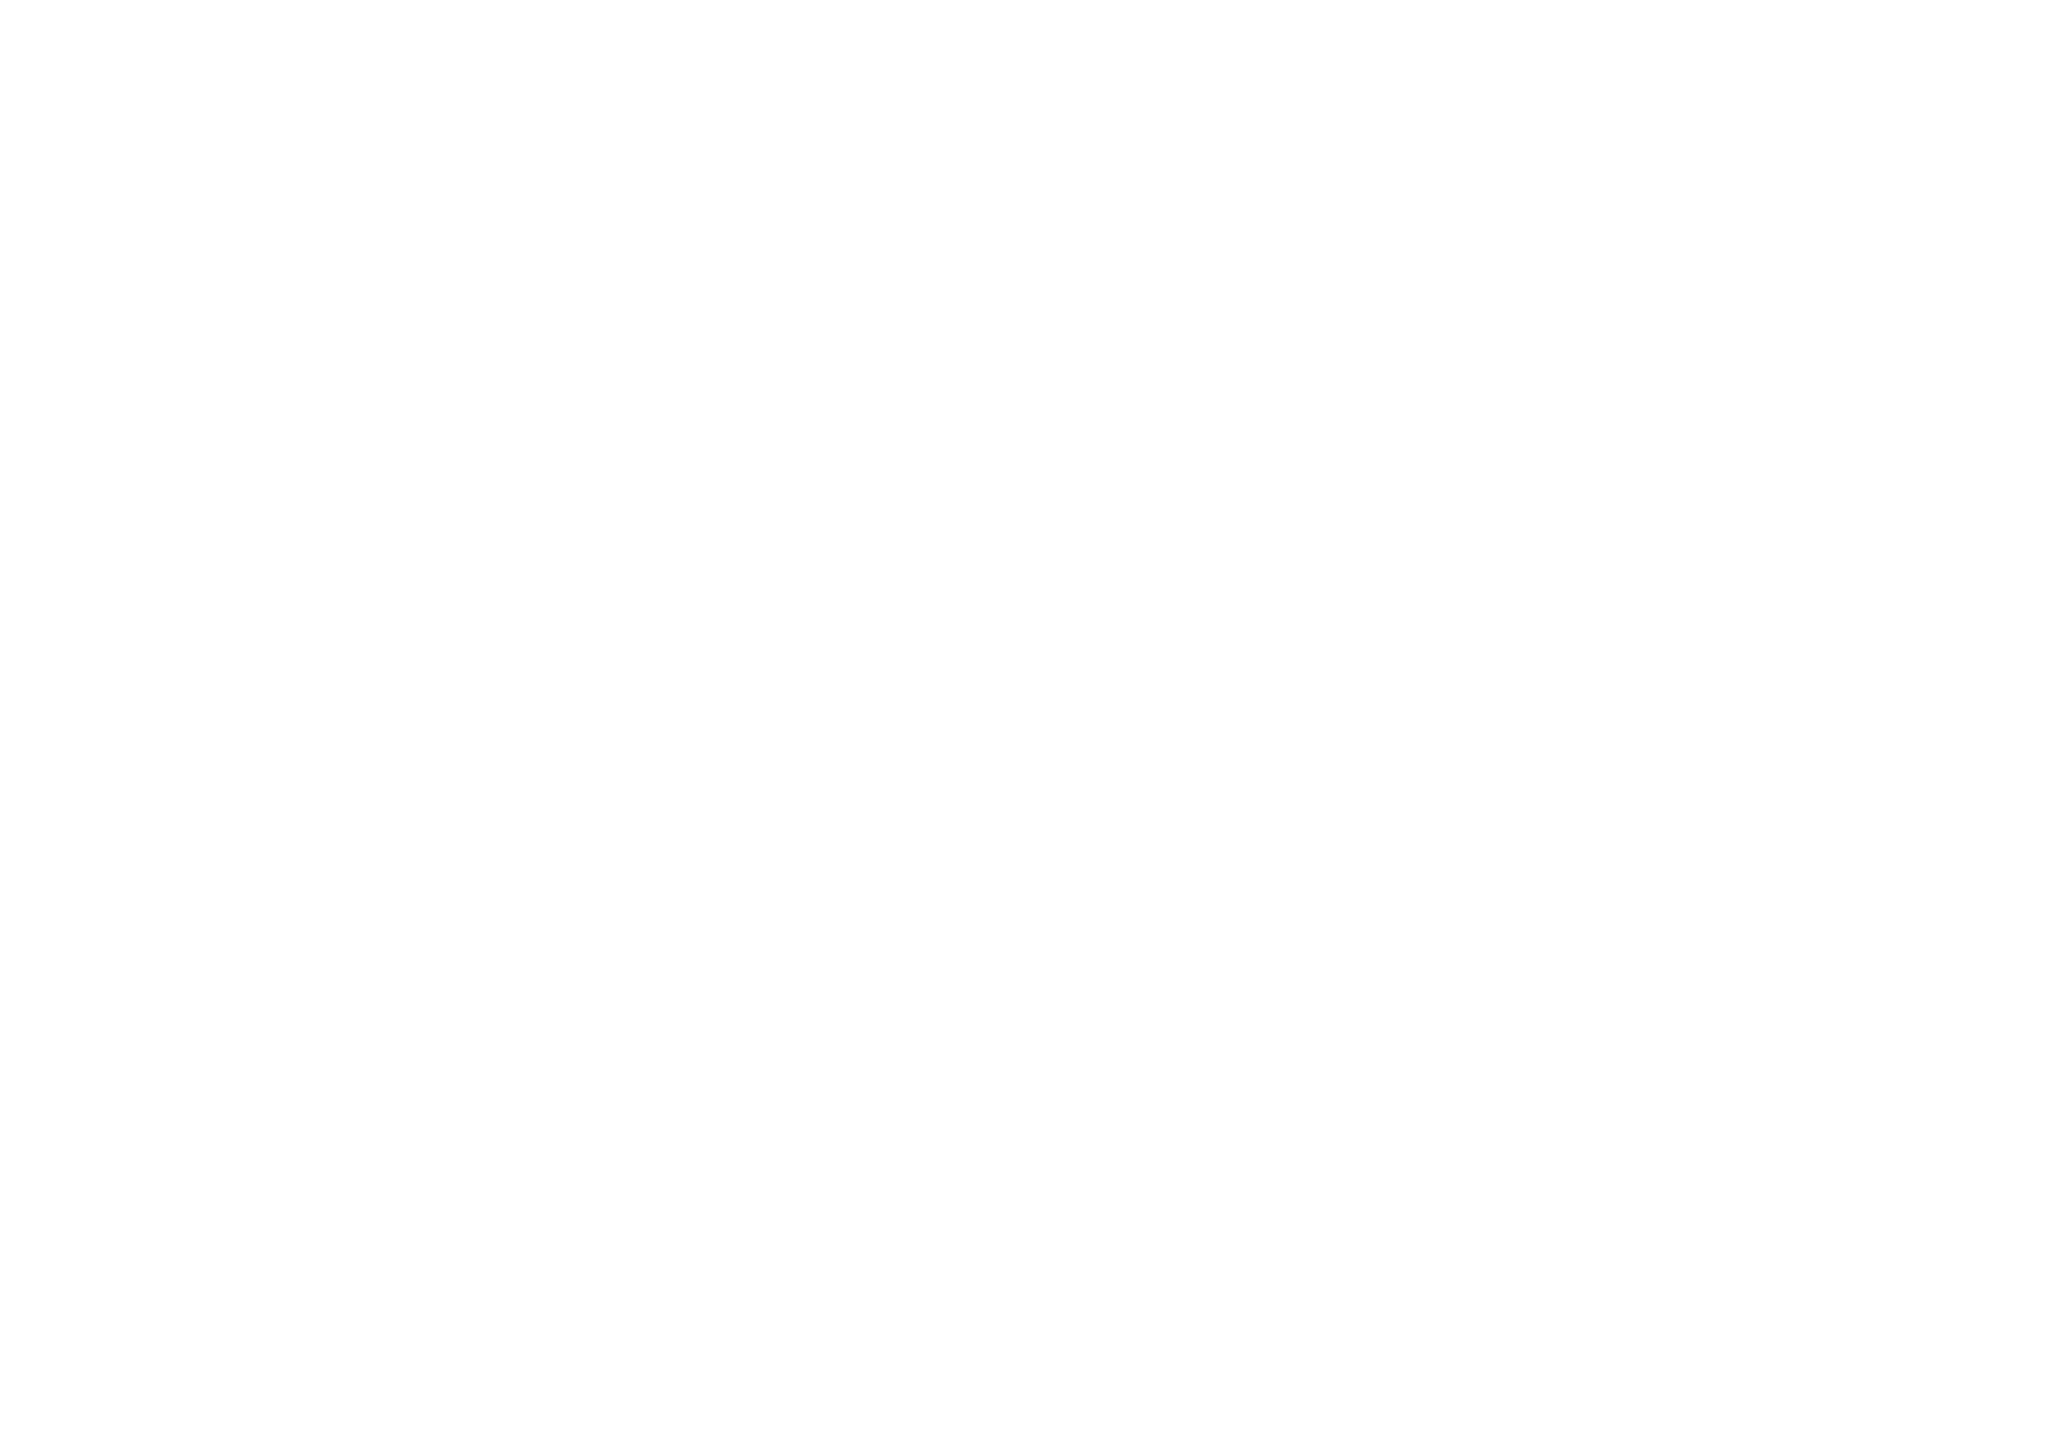
\includegraphics[width=0.90\textwidth]{cpu_branch_pred.pdf}
\end{frame}

\begin{frame}
\frametitle{Result of Pipelined RISC-V Processor Design}
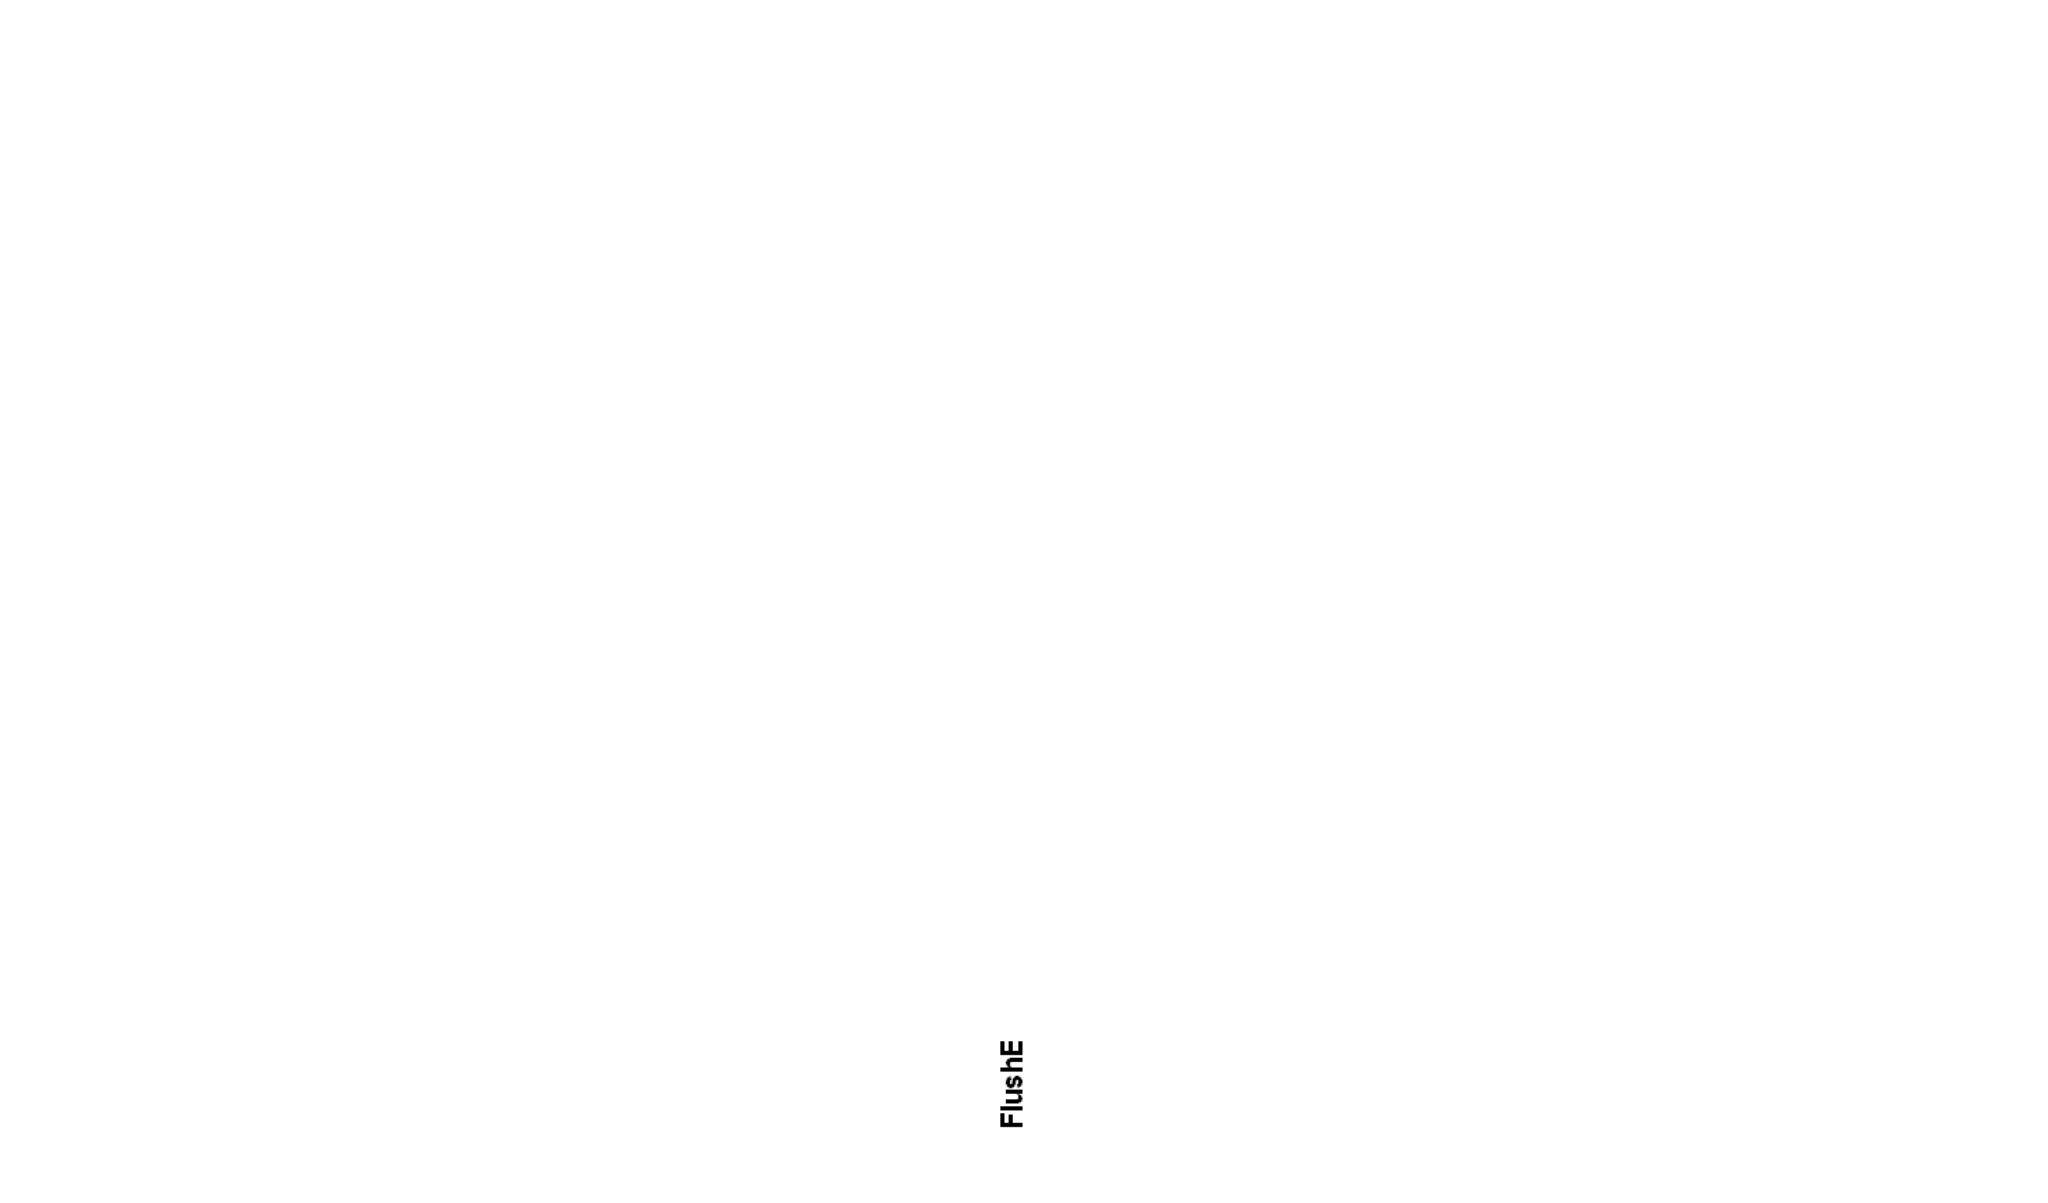
\includegraphics[width=0.95\textwidth]{cpu_final_design.pdf}
\end{frame}

\begin{frame}
\frametitle{Performance of the Designed Pipelined Processor}

\begin{itemize}
 \item What will be the maximum achievable frequency of the processor?
 \item Which stage is the slowest one?
 \item The minimum feasible cycle time is given by the slowest stage
 \item In our case, we are dealing with memory \\
       $T_C = 300$\,ns $\rightarrow$ $f_{clk\,max} = 3\,333$\,kHz \\
       if we don't consider extra cycles to fill the pipeline (no pauses
       and emptying during branches, for example) then for an ideal $IPC = 1$ \\
       $IPS = 1 \cdot 3\,333e3 = 3\,333\,000$ instructions per second
 \item The introduction of five-stage pipelined processing has led to an increase in
       throughput of $3\,333\,000 / 980\,000 = 3.4 \times$ assuming $IPC = 1$
\end{itemize}

\end{frame}

\section{Processor with External Memory}

\begin{frame}
\frametitle{Design Correspondence to a Real Processor with External Memory (for simplicity we don't consider the pipeline)}
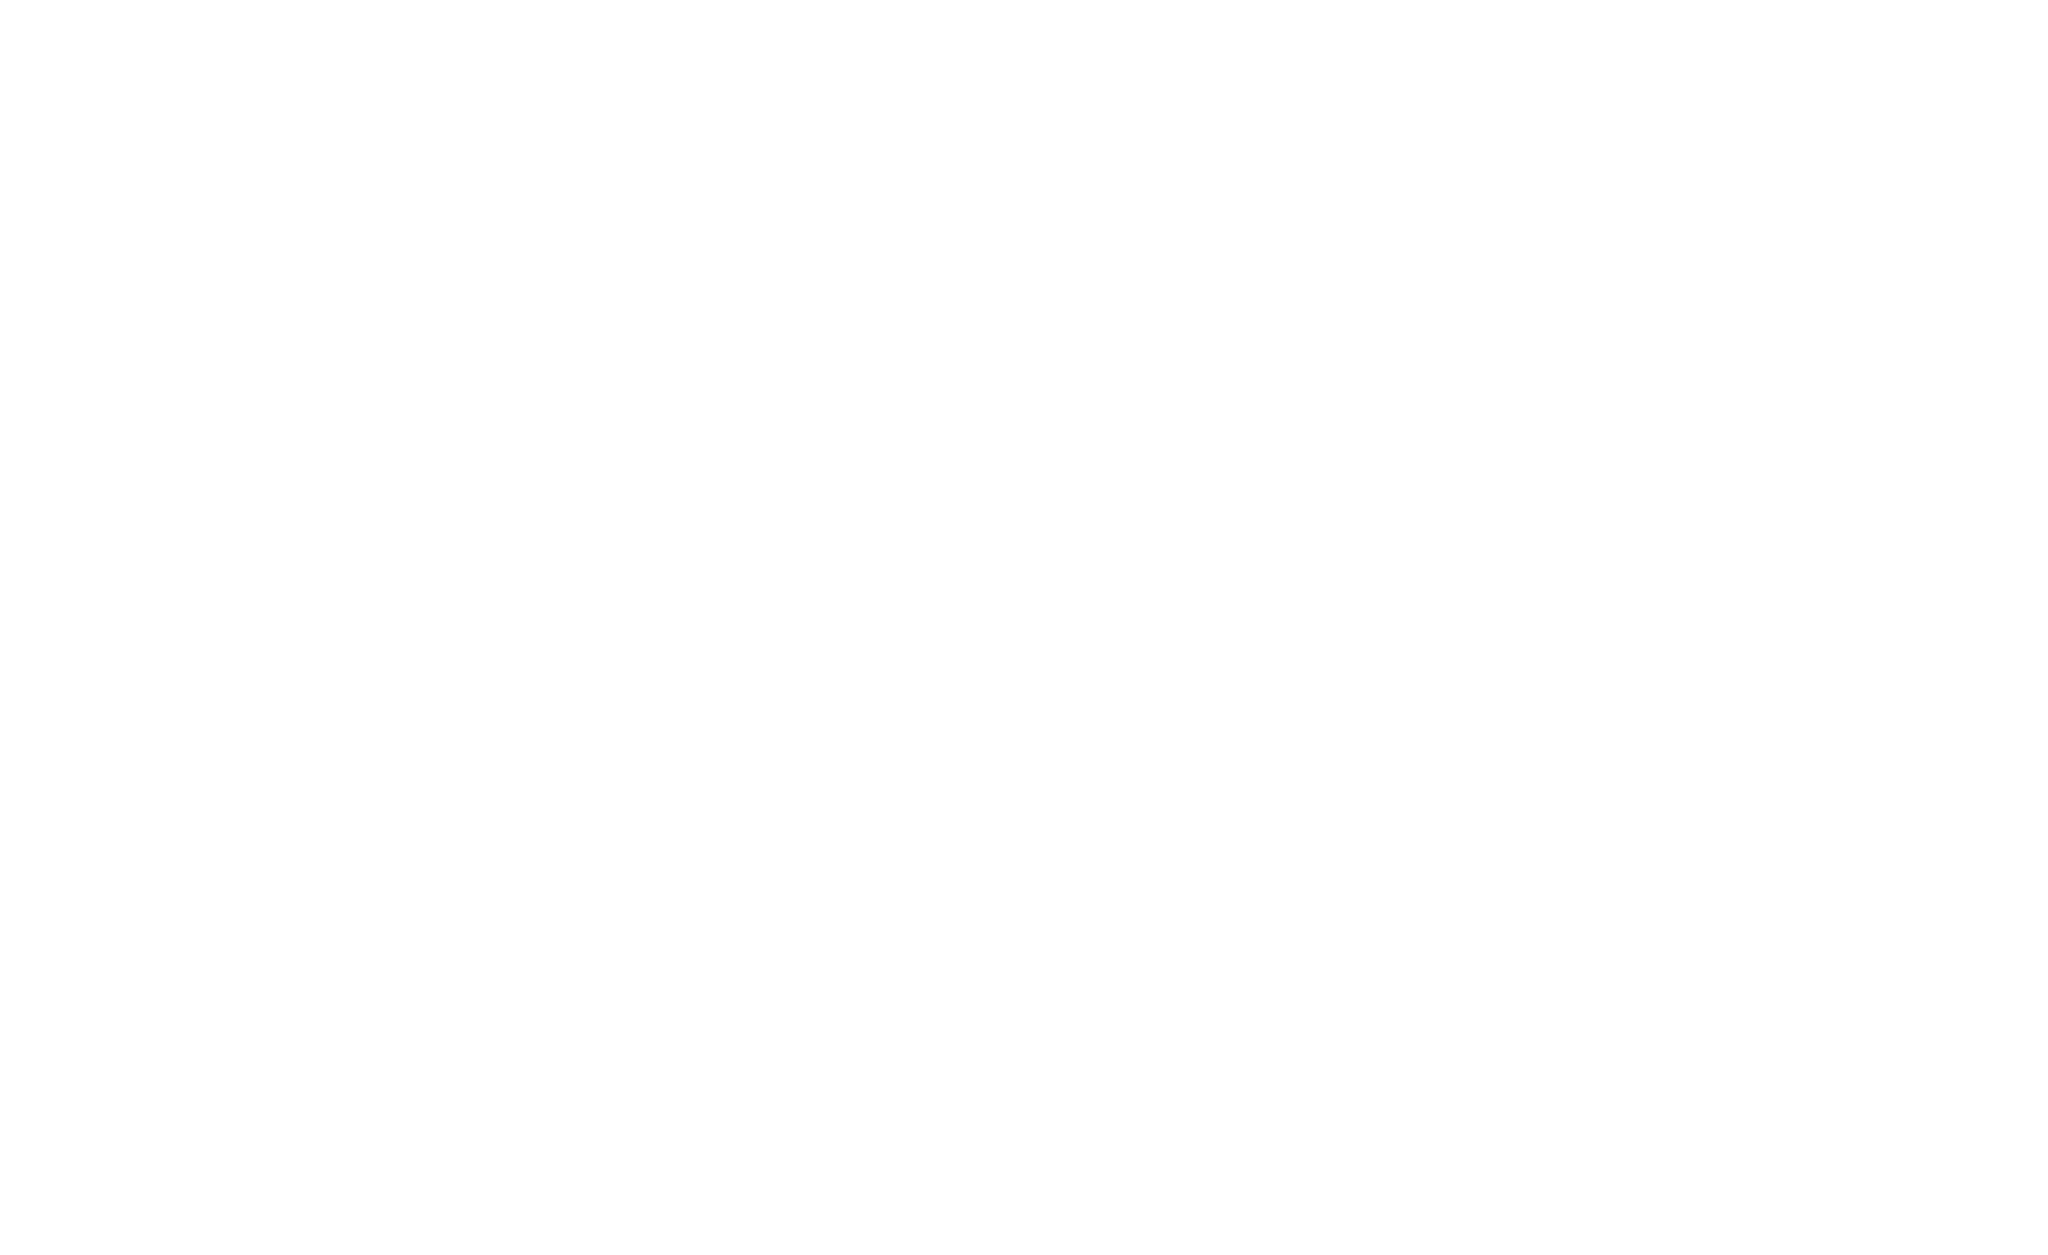
\includegraphics[width=0.95\textwidth]{cpu_design.pdf}
\end{frame}

\begin{frame}
\frametitle{Memory Is no Longer Placed Inside the Processor}
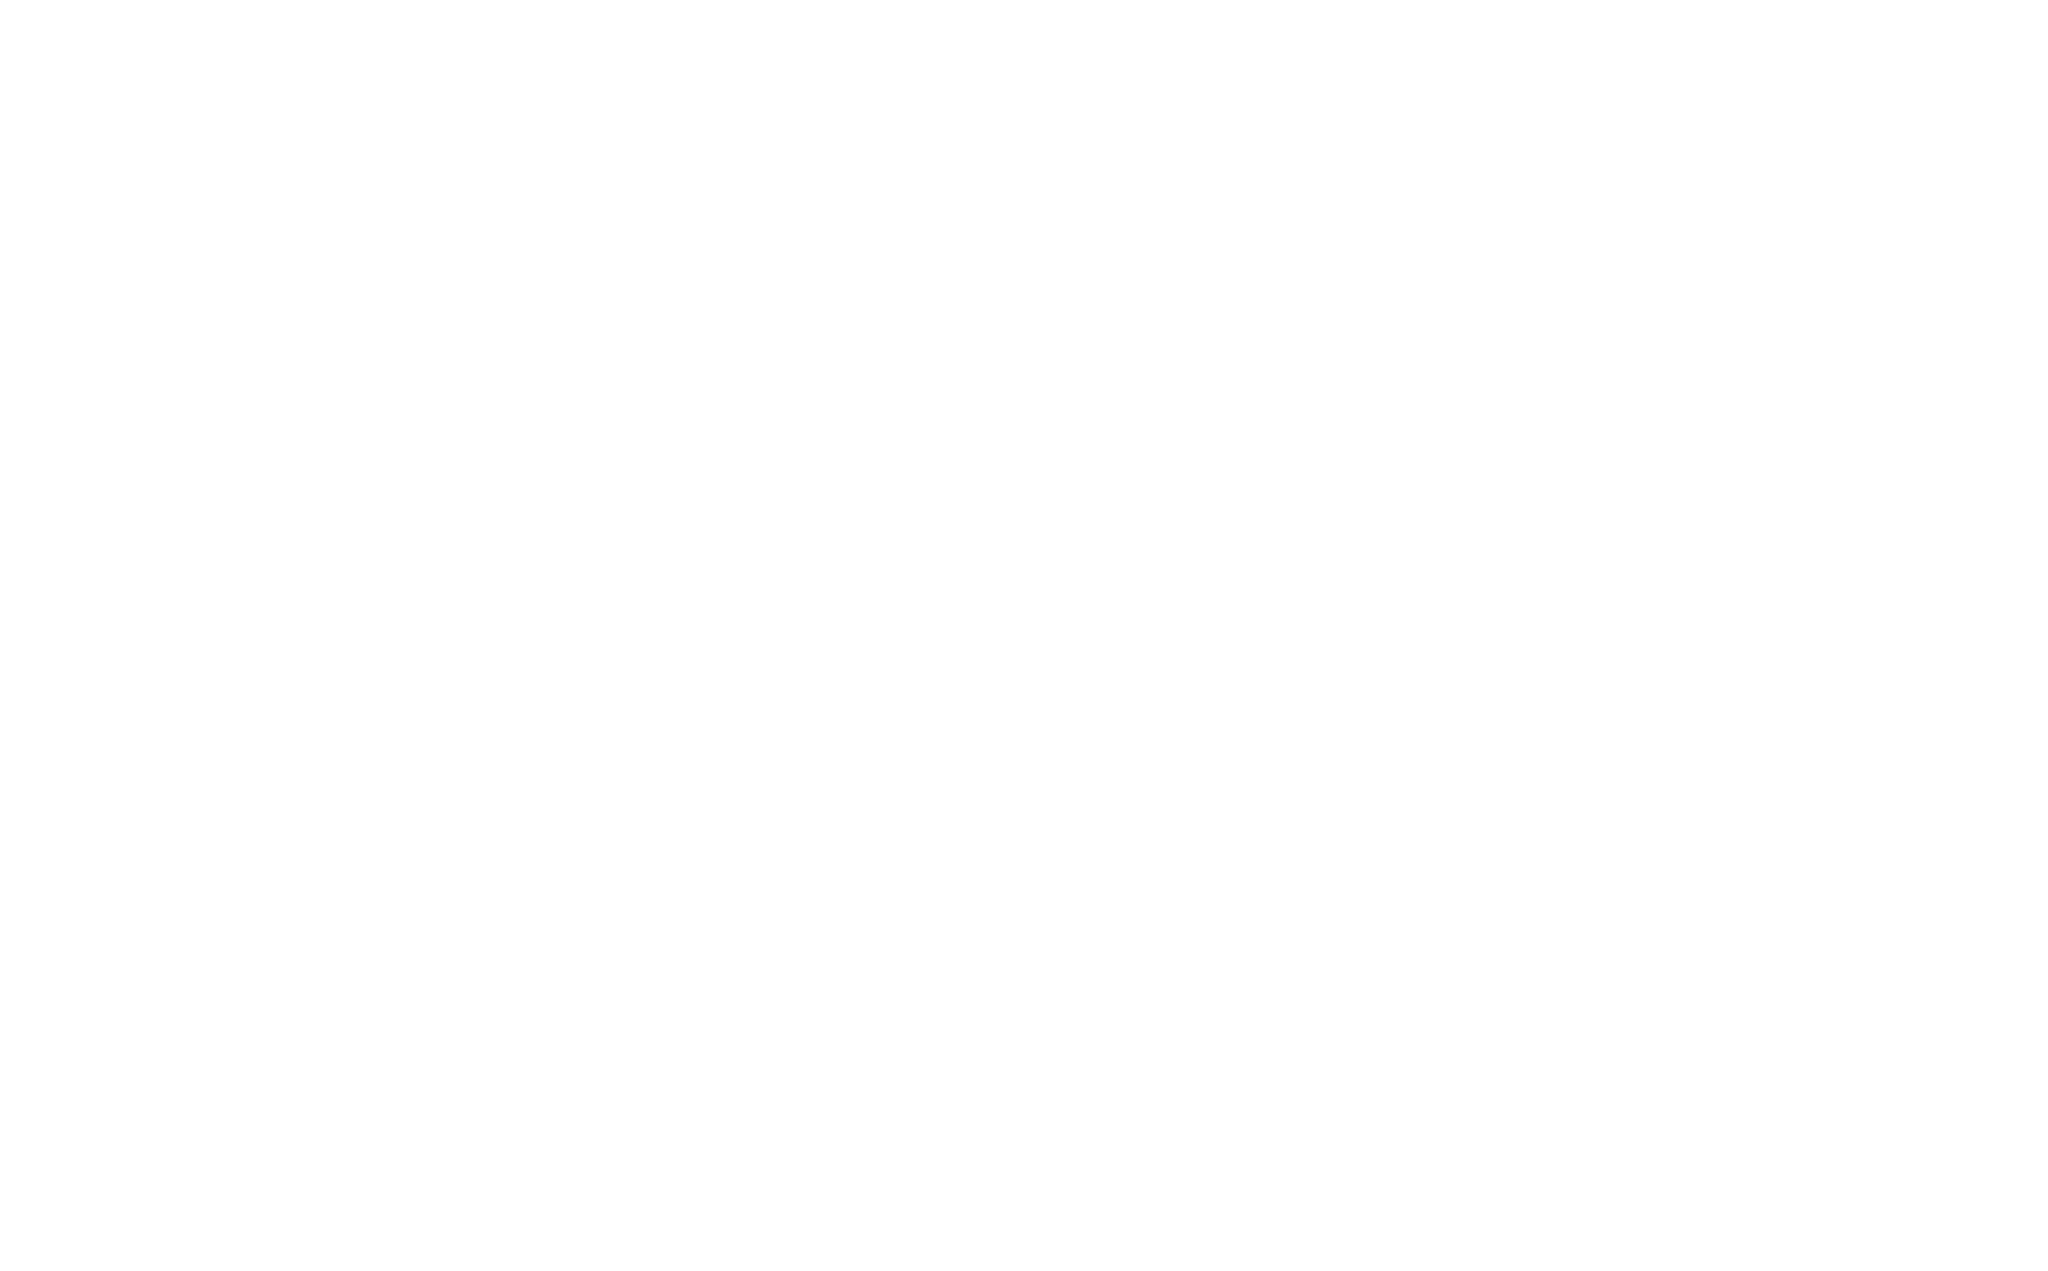
\includegraphics[width=0.95\textwidth]{cpu_design2.pdf}
\end{frame}

\begin{frame}
\frametitle{getting Back to the Original Separated CPU and Memory}
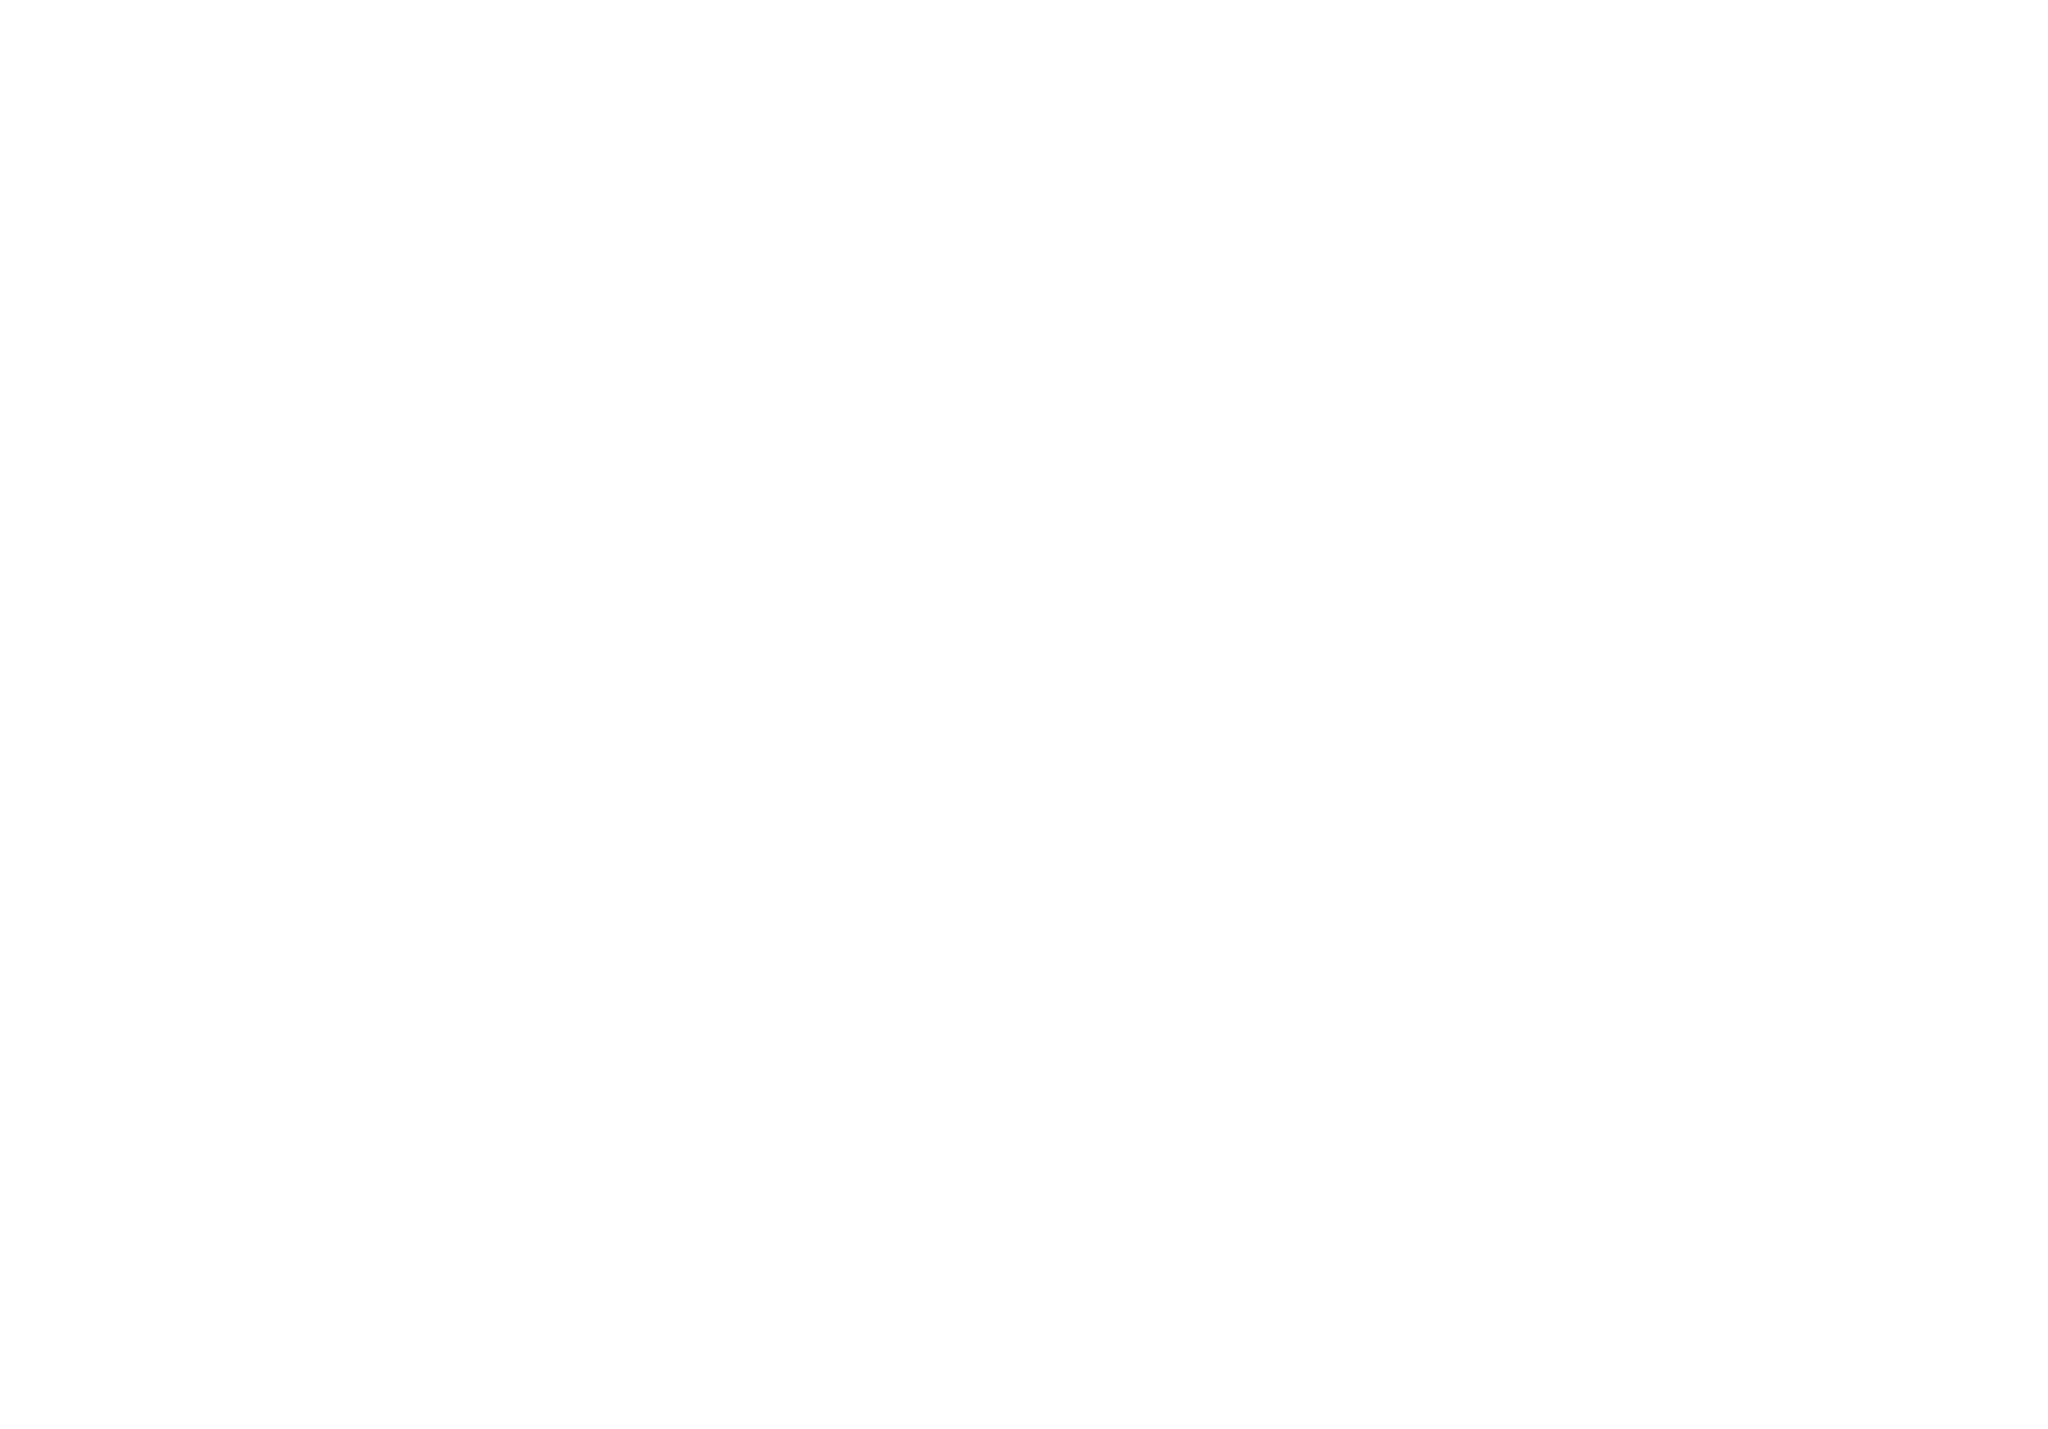
\includegraphics[width=0.85\textwidth]{cpu_design3.pdf}
\end{frame}

\begin{frame}
\frametitle{Quiz -- Which Instruction Misbehaves When Signal is Cut}
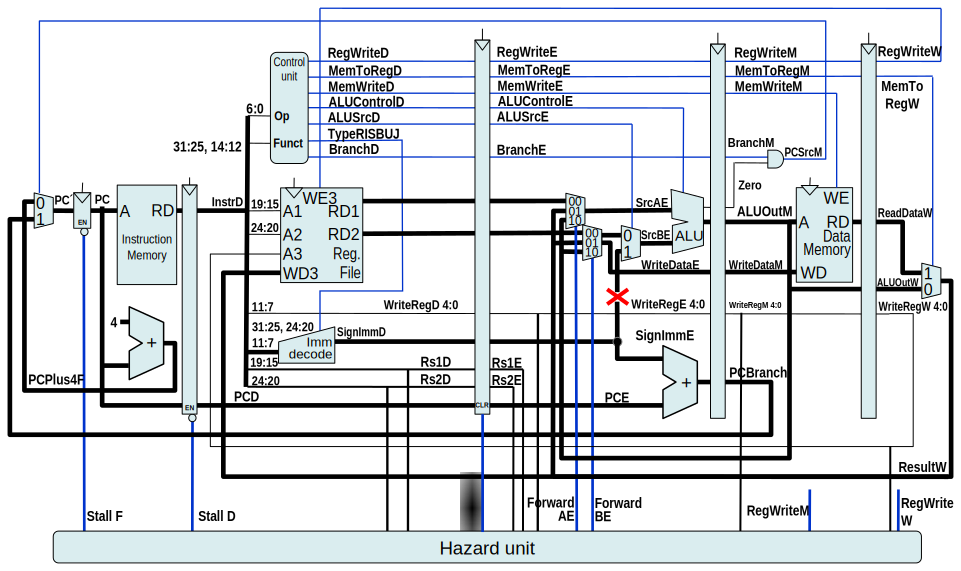
\includegraphics[width=0.95\textwidth]{cpu_final_design_bonus.pdf}

\textbf{A)} add \hfill \textbf{B)} addi \hfill \textbf{C)} beq \hfill \textbf{D)} or \hfill ?
\end{frame}

\section{Real Design Considerations and Constraints (for A Grade Adepts)}

\begin{frame}
\frametitle{Requirements for Pipeline Timing}
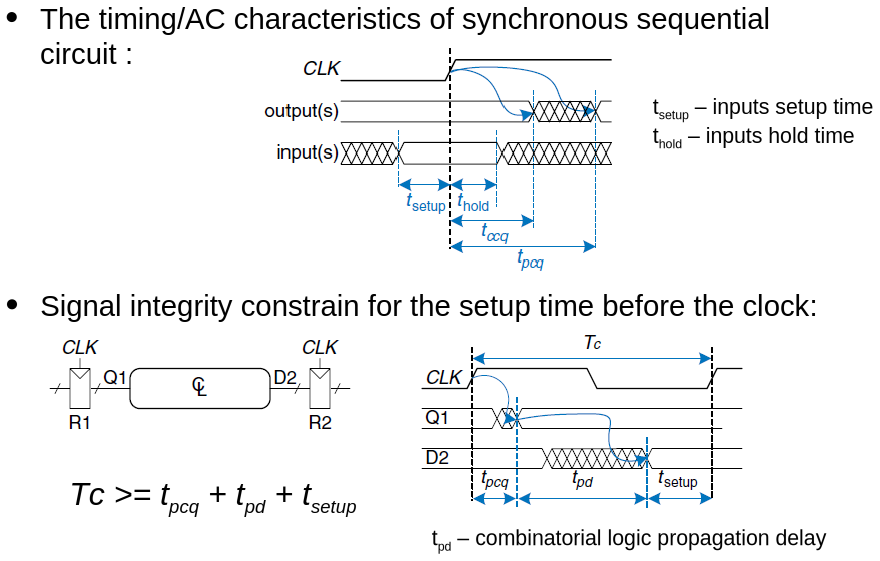
\includegraphics[width=0.95\textwidth]{pipeline_timing1.pdf}
\end{frame}

\begin{frame}
\frametitle{Requirements for Pipeline Timing}
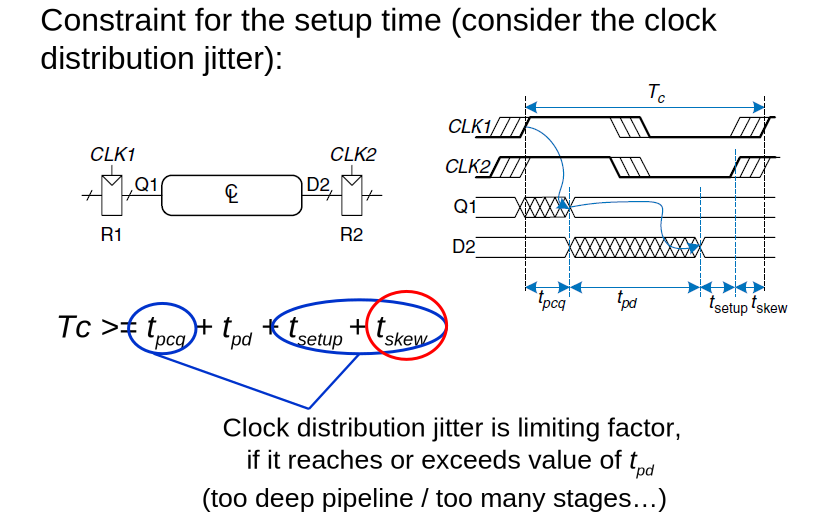
\includegraphics[width=0.95\textwidth]{pipeline_timing2.pdf}
\end{frame}

\begin{frame}
\frametitle{Clock Distribution Network Skew}
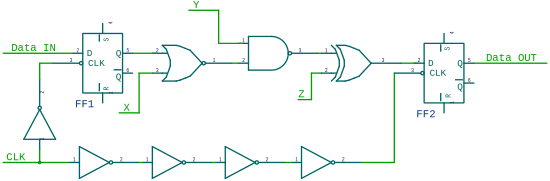
\includegraphics[width=0.9\textwidth]{clock_distribution_skew.pdf}

\begin{itemize}
 \item \textbf{Positive Clock Skew} -- clock arrives at the capturing sequential later than it arrives at the launching sequential
 \item \textbf{Negative Clock Skew} -- clock arrives at the launching sequential later than it arrives at the capturing sequential
 \item \textbf{Local Clock Skew} -- skew between any two sequentials with a valid timing path between them.
 \item \textbf{Global Clock Skew} -- clock skew between any two sequentials in the design regardless of whether a timing paths exists between them
\end{itemize}

\end{frame}

\begin{frame}
\frametitle{Clock Distribution Network -- H-tree}

{
\centering
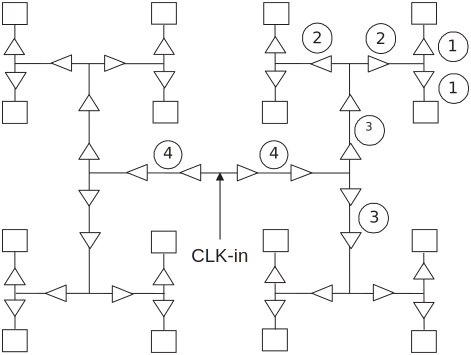
\includegraphics[width=0.6\textwidth]{clock_distribution_h_tree.pdf}
}

\vskip 2mm

source: Tawfik, S., Kursun, V.: Clock Distribution Networks with Gradual Signal Transition Time Relaxation for Reduced Power Consumption.

\end{frame}

\begin{frame}
\frametitle{Pipeline Stages Balancing}
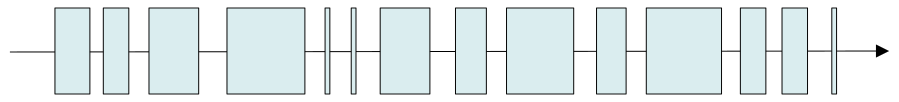
\includegraphics[width=0.85\textwidth]{pipeline_balancing.pdf}

(applies to tree based adder, multiplier, (unrolled) iterative divider..)

\begin{itemize}
 \item \textbf{Balancing}: the goal is to divide the processing into N stages in such a way, that stage propagation delays are roughly the same...
 \item The number of stages reflects preference of \underline{performance} (\underline{throughput}) versus latency.
\end{itemize}

\end{frame}

\begin{frame}
\frametitle{Superpipeline and Beyond}

\begin{itemize}
 \item Not well balanced 5-stage pipeline:
\end{itemize}

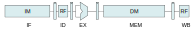
\includegraphics[width=0.85\textwidth]{pipeline_balancing2.pdf}

\begin{itemize}
 \item Deeper pipeline is result of decomposing stages into more stages
\end{itemize}

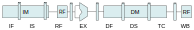
\includegraphics[width=0.85\textwidth]{pipeline_balancing3.pdf}

\begin{itemize}
 \item It allows CPU to work at higher frequencies but introduces many problems as well...
 \item Complex forwarding, more pipeline stalls, hazards need to be solved by complex logic
\end{itemize}

\end{frame}

\begin{frame}
\frametitle{Superpipeline and Beyond}

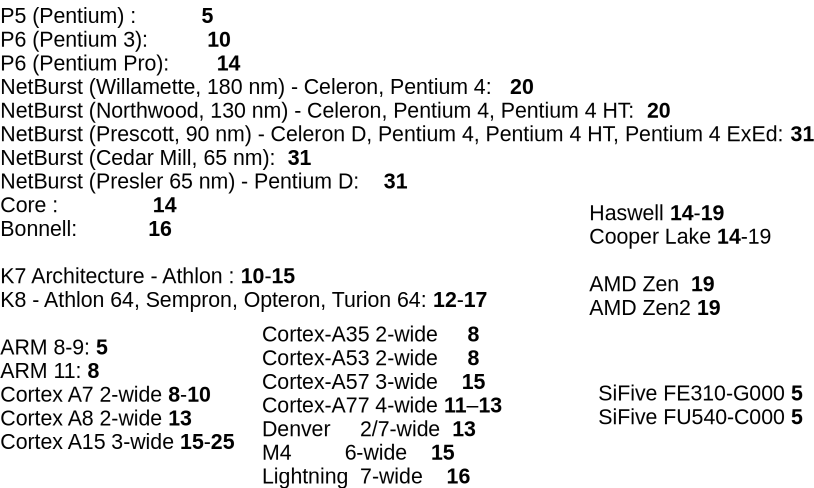
\includegraphics[width=0.95\textwidth]{pipeline_today_depths.pdf}

The Optimum Pipeline Depth for a Microprocessor: {\tiny \url{http://citeseerx.ist.psu.edu/viewdoc/download?doi=10.1.1.93.4333\&rep=rep1\&type=pdf}}

\end{frame}

\end{document}

